\chapter{In Vivo Deployment for Industrial Environments}\label{c3}

% Present your internship experiences
%\textbf{Currently contains \the\numexpr\getpagerefnumber{c3}-\getpagerefnumber{c2}\relax  pages.}
%\textbf{20 pages}
% ~ 10 pages




\section{Introduction}

%\subsection{Motivation}

\begin{marginfigure}%
  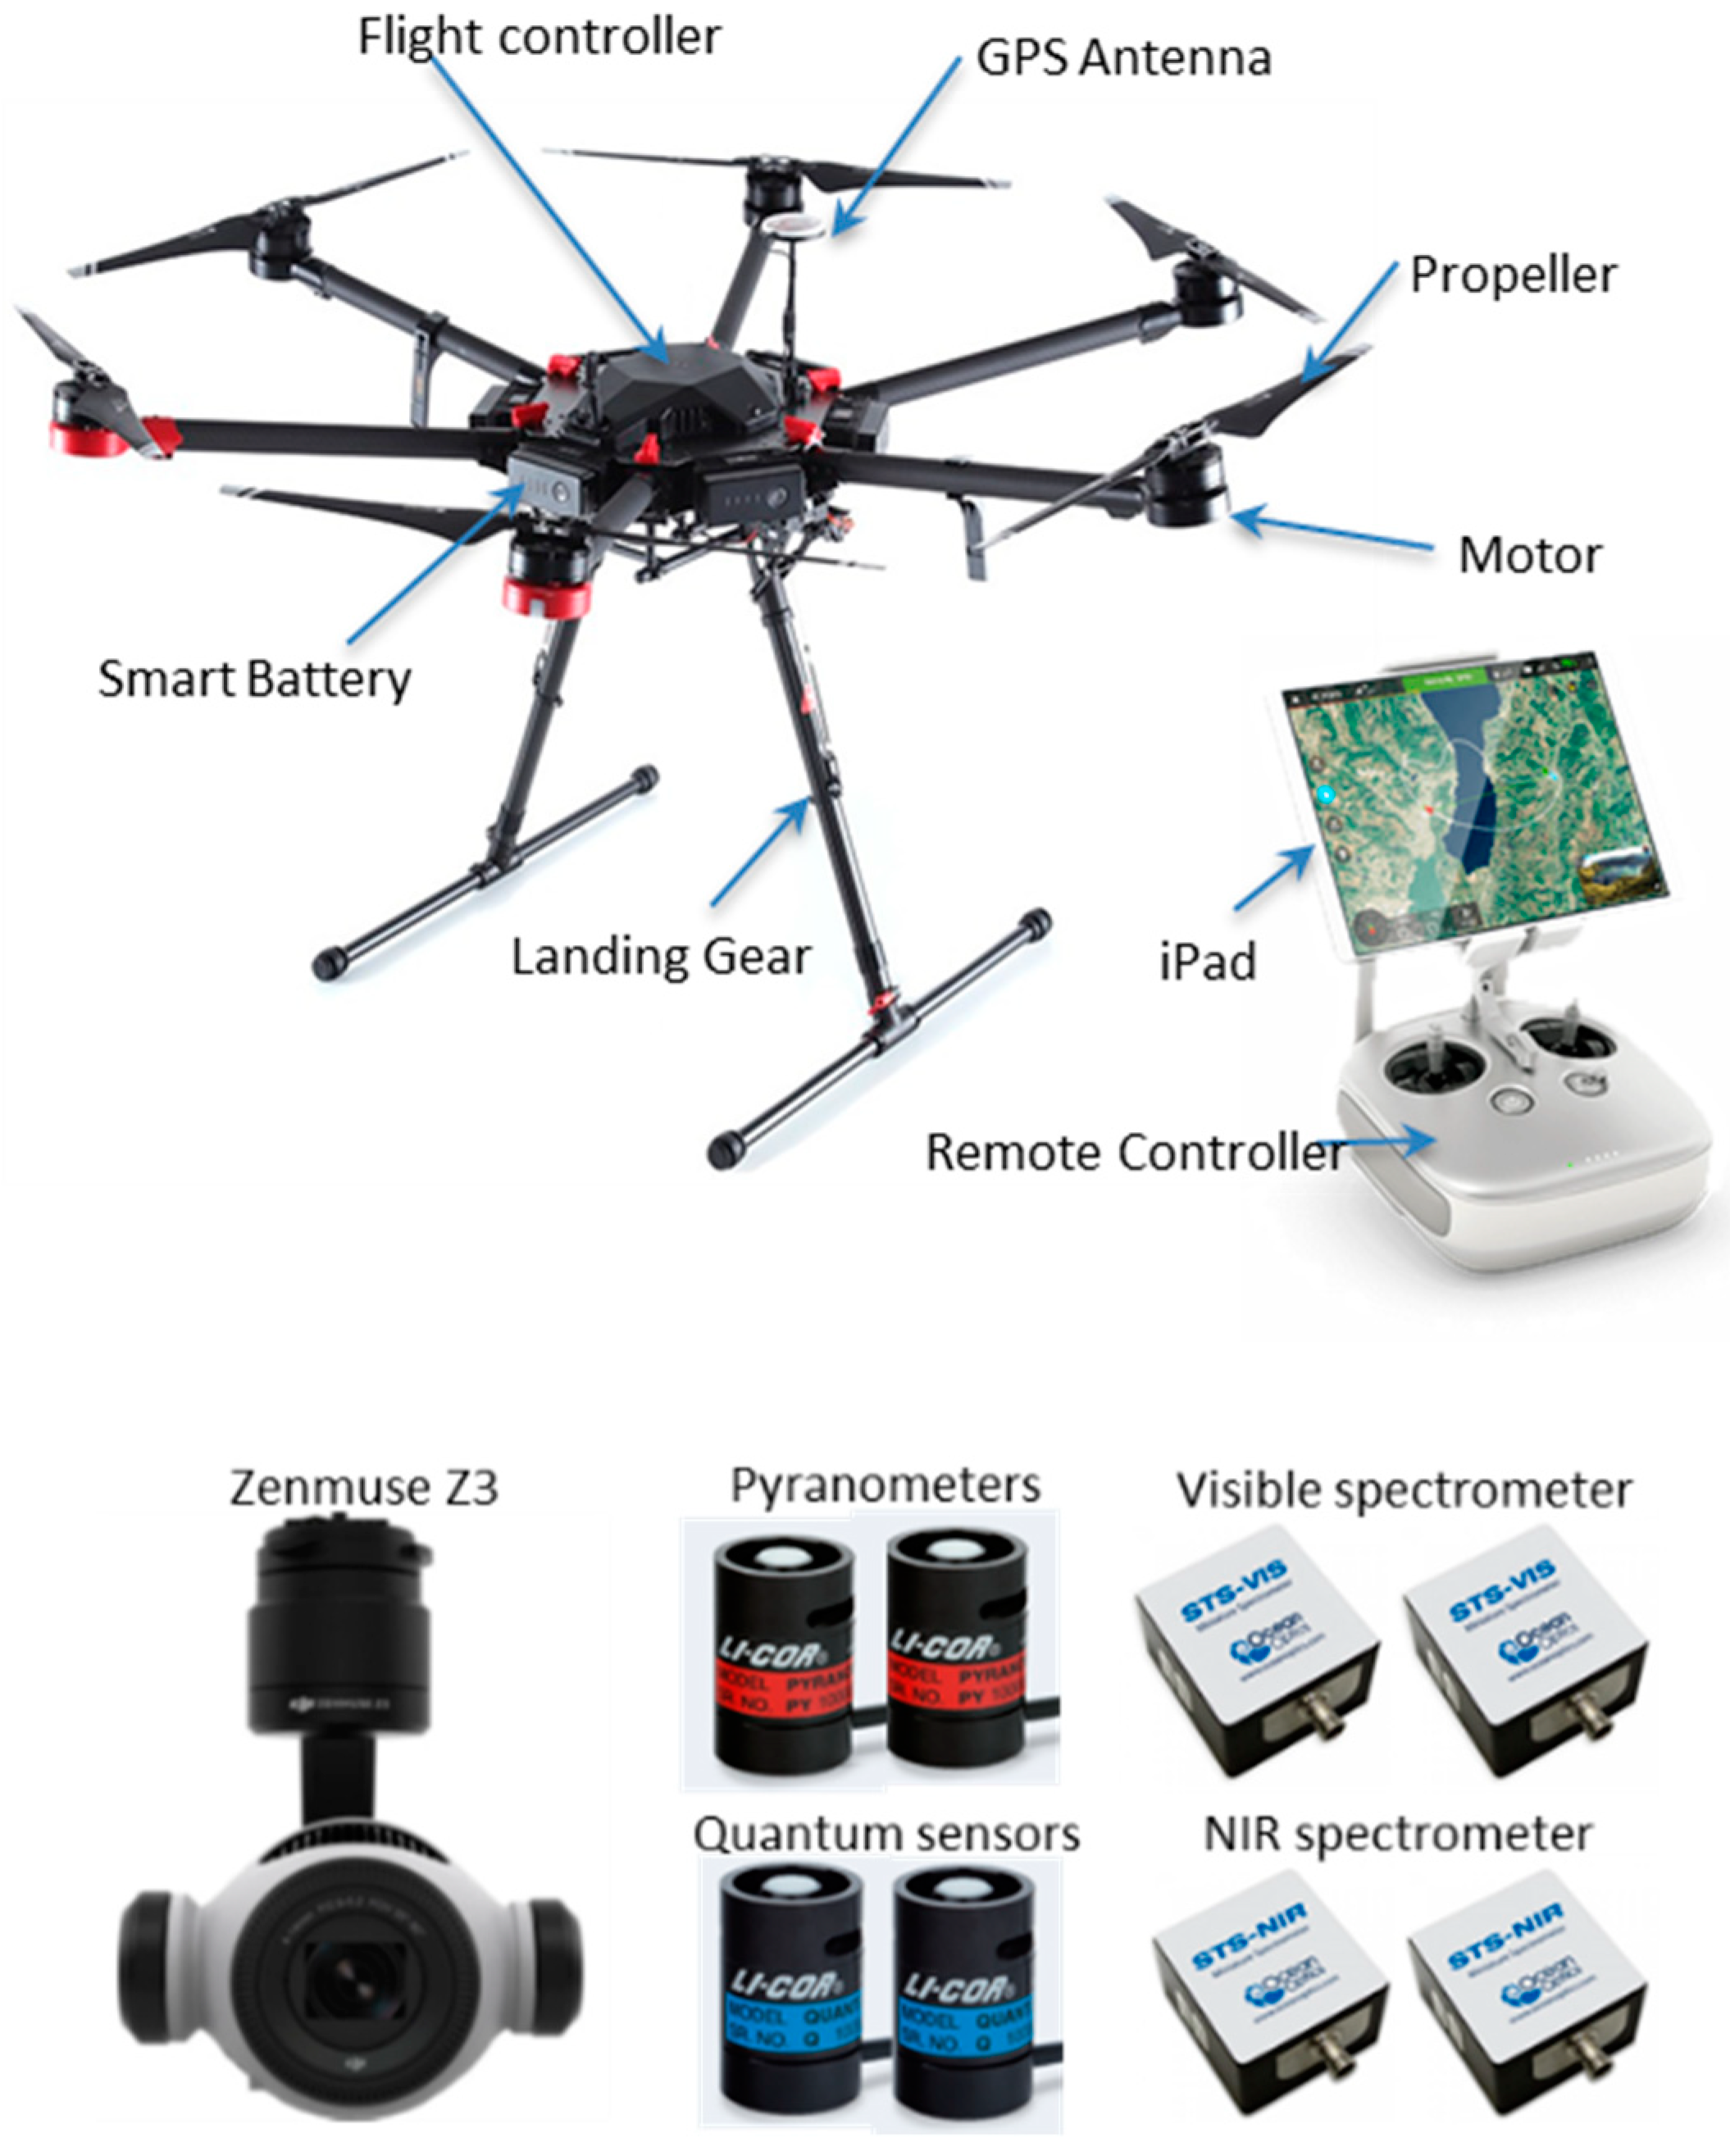
\includegraphics[width=5cm]{images/stage_sota/albedo_drone.png}
  \caption{example of a remote-sensing vehicle: The DJI's Matrice 600 for Measuring Land Surface Albedo \cite{land_surface_albedo}}
  \label{fig:dji}
\end{marginfigure}
UAVs provide us with a novel way to capture data; they help us to gain a perspective of the Earth that is simply not possible with instruments that are based on the ground. In contrast with the platforms of manned aircraft and satellite, the UAV
platform holds many promising characteristics \cite{xiang_xia_zhang_2020}: flexibility, efficiency, high-spatial/temporal resolution, low cost, easy operation, etc., which make it an effective complement to other remote sensing platforms and a cost-effective means for remote sensing. As a result, low-cost, light-weight UAVs have been used extensively within research for more than a decade to measure, for instance, air quality, mapping of 3D geodata and remote sensing within agriculture \cite{metrology_survey}. However, until recently, UAVs were build with a single purpose and with one particular sensor on board.


From about 2010, the stability, flight duration, and load capacity of UAVs increased significantly with the development of flight-control and battery technology, which enable more sensor varieties (optical sensor, lidar or radar) to be mounted on smaller UAVs \cite{uav_components}. Figure \ref{fig:dji} alongside demonstrates this: a multi-rotor based UAV platform was developed and tested for measuring land surface albedo and spectral measurements at user-defined spatial, temporal, and spectral resolutions. This drone onboards an RGB camera and a set of four downward pointing radiation sensors.


\begin{marginfigure}%
  \vspace{0.3cm}
  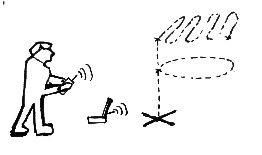
\includegraphics[width=4cm]{images/intro/outputonlinejpgtools.jpg}
  \caption{An environment for outdoor deployments.}
  \label{fig:outdoors}
\end{marginfigure}

% {c3_thesisgoal}
In line with the thesis goal, we pay attention to the interplay between smart systems, and the real-world deployment of a UAV. The carrier drone aids in streamlining the data collection process, by automating different fly-by procedures, safeguards, and scheduling the data collection. Two payloads are tested in outdoor flight, for atmospheric data and vibration data, and the sensors used in these tests are evaluated. In this way, onboard systems can aid with the practitioner’s task.




\pagebreak

\section{Related Work}

In the literature, there is increasing reference made to the potential of using UAVs as autonomous or semi-autonomous operating data acquisition platforms, often referred to as Mobile Sensing Platforms (MSPs) \cite{sørensen_jacobsen_hansen_2017} \cite{metrology_survey}. They can be equipped with state-of-the-art measurement instruments offering extremely high resolution and are ideally suited to 
% NEED TO HAVE A VALID REASON!!
access otherwise prohibitingly inaccessible locations or to operate in hostile environments that would be lethal to the human operator.

\Copy{mobile_mapping_scope}{
The field scope is restricted to mobile sensing upon UAVs. Furthermore, the focus is in data inspection and data gathering in outdoor inspections as opposed to inspecting underground and pipeline plants, as well as urban spaces, as opposed to powerplants, solar farms, wind farms, or precision agriculture. As a result, we have restricted our investigations to two sectors of research: remote sensing research and structural inspections. }
%{mobile_mapping_scope}
%\textbf{~4 pages}
% \begin{itemize}
%     \item How did researchers tackle the challenge at hand in the past
%     \item What are the trade-offs of the different alternatives and why did you choose a particular one
%     \item How does your contribution relate to prior work
%     \item Also includes technical state of the art, i.e. available technologies and technologies used in this work
% \end{itemize}

\subsection{Remote Sensing Research}
% \textbf{An overview of Mobile Sensing}


% {mobile_mapping_field}
We see great growth in mobile mapping research, that is “the acquisition of spatiotemporal phenomena by using a mobile multi-sensor platform” \cite{mobile_mapping}. The UAV is a platform that greatly simplifies research. One such field remote sensing, the acquisition of information about an object or phenomenon without making physical contact with the object \cite{remote_sensing}. Recently, UAVs have enabled research towards contact sensing, for the acquisition of information in direct contact with the object \cite{sensor_placement_uav}, on a platform that serves for optimal sensor placement \cite{sensor_placement_uav} \cite{stewart_chang_sudarchan_becker_huang_2016}.

\begin{marginfigure}%
  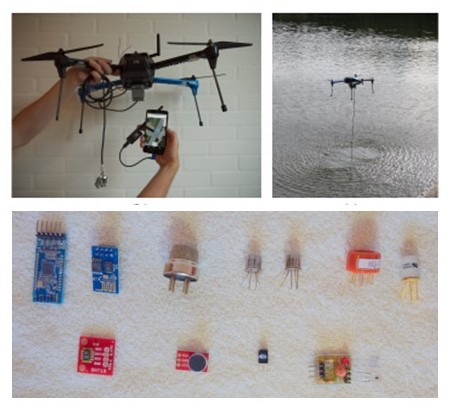
\includegraphics[width=5cm]{images/stage_sota/arduino_drone.jpg}
  \caption{A low-cost, open-source, modular sensor platform \cite{sørensen_jacobsen_hansen_2017}.}
  \label{fig:msp}
\end{marginfigure}

\Copy{mobile_mapping_advantages}{
In contrast with other aerial platforms like manned aircraft and satellite, the UAV
platform holds many promising characteristics \cite{xiang_xia_zhang_2020}: flexibility, efficiency, high-spatial/temporal resolution, low cost, easy operation, etc., which make it an effective complement to other remote sensing platforms and a cost-effective means for remote sensing. As a result, low-cost, light-weight UAVs have been used extensively within research for more than a decade to measure, for instance, air quality, mapping of 3D geodata and remote sensing within agriculture \cite{metrology_survey}. However, until recently, UAVs were build with a single purpose and with one particular sensor on board.
}

\cite{sørensen_jacobsen_hansen_2017} \hspace*{0.3cm} \textit{\citename{sørensen_jacobsen_hansen_2017}{author}}
\hspace*{0.5cm}
propose a multi-sensor platform based on commercial off-the-shelf components that provides a modularized sensor system and data acquisition infrastructure. This "Mobile Sensor Platform" (Figure \ref{fig:msp}) is a commercial quadcopter that allows for attaching external sensors and relaying the data back to a ground station using a telemetry communications link. The platform supports a simple and expandable interface for attaching custom sensors to the UAV, overcoming the limitation of single-purpose platforms which are costly to convert for other tasks.  

%— La détection des gaz atmosphériques, par exemple la surveillance du climat, la détection de la pollution, la volcanologie, la surveillance des sites industriels et l’évaluation des scènes dangereuses, comme la surveillance des feux de forêt. La détection de gaz par drone a aussi été utilisée pour échantillonner l’humidité au niveau de la mer (capteur utilisé : capteurs à oxyde métallique). 

Unmanned aerial vehicles have been shown to be useful for the installation of wireless sensor networks. Wireless sensor network (WSN) technology refers to a group of sensors used for monitoring and recording the physical conditions of the environment and organizing the collected data at a central location \cite{metrology_survey}. Sensor nodes can be placed more accurately  with the development of autonomous aerial robots capable of physically interacting with the environment.

% [ PHYSICALLY INTERACTING ]

% NO TIME
% \cite{vasek_atter_rizo_nam_kortvelesy_kaufman_das_kumar_2017} \hspace*{0.3cm} \textit{\citename{vasek_atter_rizo_nam_kortvelesy_kaufman_das_kumar_2017}{author}}
% \hspace*{0.5cm} present a sUAS capable of autonomously deploying, transporting, and retrieving a novel lightweight probe. 

\begin{marginfigure}%
  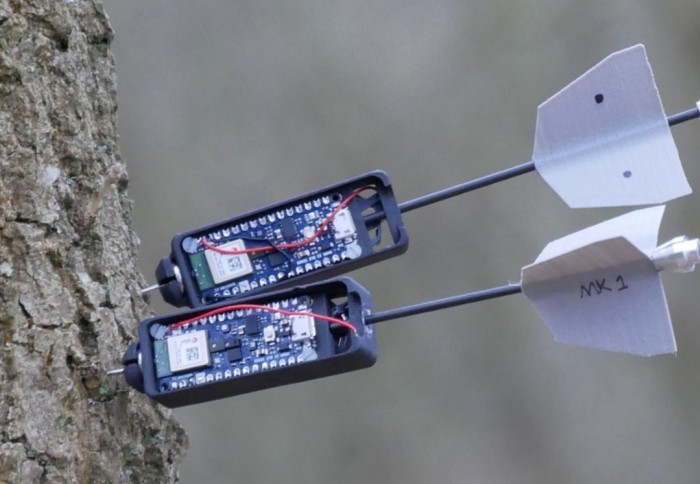
\includegraphics[width=4cm]{images/stage_sota/arrow.jpg}
  \caption{Impulsive launching of sensors to monitor the health of forests \cite{sensor_placement_uav}}
\end{marginfigure}

\cite{sensor_placement_uav} \hspace*{0.3cm} \textit{\citename{sensor_placement_uav}{author}}
\hspace*{0.5cm} present a novel method for aerial sensor placement in hazardous environments. This method is applied to Wireless Sensor Network deployment. The proposed system does not require direct physical interaction to accurately place sensors which brings significant advantages in cluttered environments and in overall operational safety.


% HM-10 (Bluetooth), ESP8266 (WiFi),
% MQ-135 (air quality: NH3, NOx, alcohol, benzene, smoke and CO2), Figaro TGS2600 (air quality:
% methane, CO, ethanol, hydrogen and iso-butane), Figaro TGS2602 (air quality: ammonia, hydrogen
% sulfide, toluene, ethanol and hydrogen), MQ-7 (air quality: CO), Figaro TGS2442 (air quality: CO),
% SparkFun 13683 (humidity and temperature), SparkFun 12758 (electric microphone), IR (infrared
% light) receiver and IR receiver module.

% NO TIME
% In industrial sensing cases and other field studies where precise placement of the sensors is required. For example, the usage of
% WSNs in oil rigs and wind farms has been demonstrated in the field to reduce their high maintenance costs.



% \begin{figure*}[h]
%     \centering
%     \includegraphics[width=8cm]{images/application_domains.png}
%     \caption{A survey that lists application areas as functionalities within the two application domains considered.
% WAN = Wireless Access Networks *
% RS = Remote Sensing *
% RTM = Real-Time Monitoring
% SAR = Search and Rescue
% GL = Goods Delivery/Logistics
% INT = Surveillance
% SI = Structural Inspection *
% }
% \end{figure*}


\subsection{Structural Inspections with UAVs}
%— inspections de ponts (capteurs utilisés :caméras HD, de capteurs de proximité et caméras thermiques). 
% [ GENERALLY, STRUCTURAL INSPECTIONS ]

\cite{zhou_gheisari_2021} \hspace*{0.3cm} \textit{\citename{zhou_gheisari_2021}{author}}
\hspace*{0.5cm} explore peer-reviewed bibliographic databases and offer an interesting picture of the last 10 years. A growing number of publications are identified, and the publications are classified by \citename{zhou_gheisari_2021}{author} into five main topic categories: building inspection, damage assessment, site surveying and mapping, safety inspection and progress monitoring.


\begin{marginfigure}%
  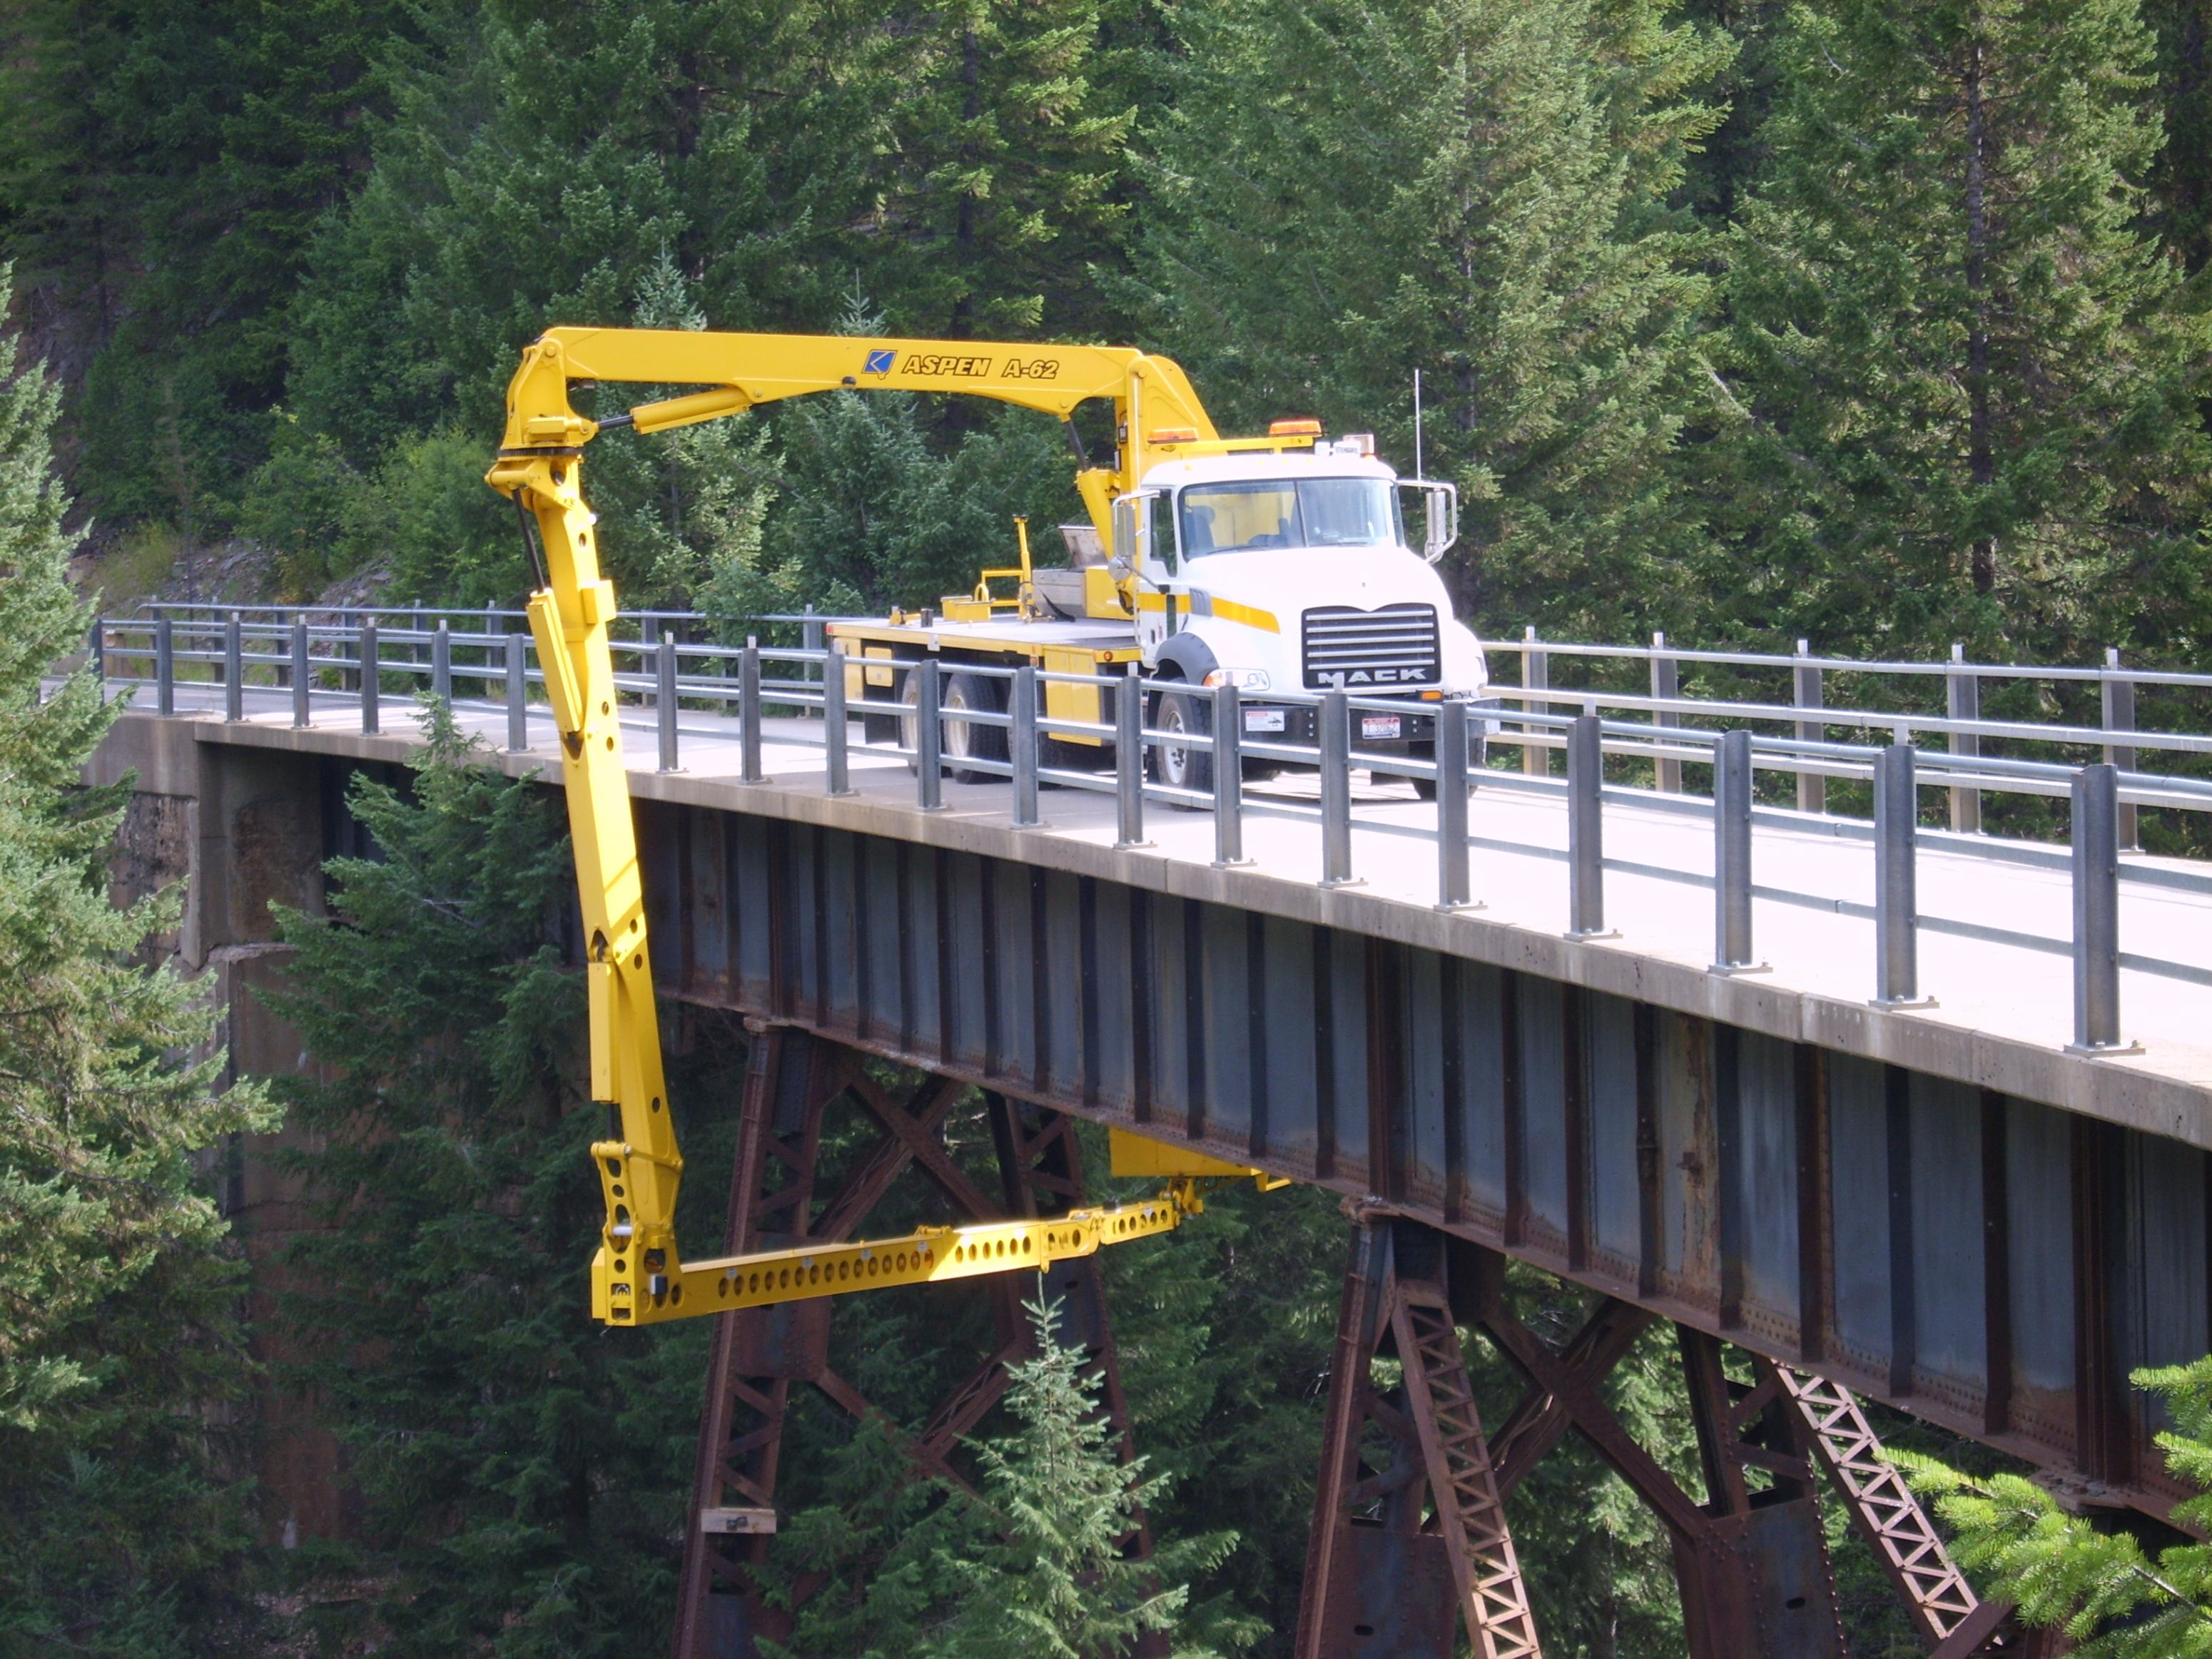
\includegraphics[width=4cm]{images/stage_sota/snooper.jpg}
  \caption{Bridge inspections with a snooper truck \cite{drone_vs_snooper_2016} (\citedate{drone_vs_snooper_2016}).}
  \label{fig:snooper}
\end{marginfigure}


Drones are a disruptive technology regarding the structural assessment for reinforced concrete bridges \cite{drone_vs_snooper_2016}. Inspectors used to employ ladders, scaffolding, or lifters to reach the parts of beams and piers of the bridge that are not easily accessible. In contrast to inspections done by snooper trucks(Figure \ref{fig:snooper}), the inspection detail that UAS provide effectively replicates some of the detail learned through the use of snoopers , without the traffic control requirements, and at significantly lower cost in terms of equipment and traffic control needs \cite{drone_vs_snooper_2016}. UAS can provide both infrared and 3D modeling detail of bridges, effectively identify concrete delamination, cracks, rebar corrosion, topographic mapping detail and other visual inspection. 
\begin{marginfigure}
    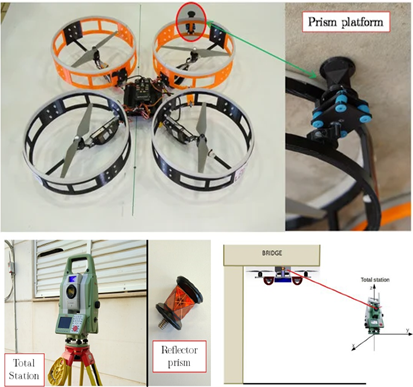
\includegraphics[width=3.8cm]{images/stage_sota/uav_prism.png}
    \caption{Bridge inspections, with a Laser Prism. \cite{feng_casero_gonzález_2019}}
\end{marginfigure}
%[width=5cm]
%[decodearray={.1 .5 .5 .5 .5 .5}] #green
\cite{feng_casero_gonzález_2019} \hspace*{0.3cm} \textit{\citename{feng_casero_gonzález_2019}{author}}
\hspace*{0.5cm} affect direct contact of the sensor or device with the bridge surfaces. Structural inspections of the internal state of a bridge require the measurements of beam deflections with direct contact. An operator manually places a reflector prism attached to a pole in contact with different points at the beam and then measures the position of the prism with a laser total station. 

\begin{marginfigure}
    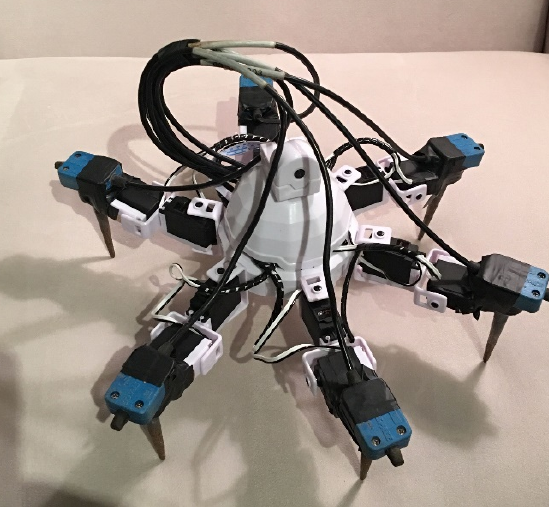
\includegraphics[width=4cm]{images/stage_sota/geophone_drone.png}
    \caption{100 Hz geophones plus recording electronics attached on a 3DR Solo Quadcopter drone.  \cite{stewart_chang_sudarchan_becker_huang_2016}}
\end{marginfigure}

\cite{stewart_chang_sudarchan_becker_huang_2016} \hspace*{0.3cm} \textit{\citename{stewart_chang_sudarchan_becker_huang_2016}{author}}
\hspace*{0.5cm} design and test an unmanned aerial vehicle with seismic sensing capabilities. The seismic sensing platform consists of four 100 Hz geophones and recording electronics. This is attached to a 3DR Solo Quadcopter drone. The geophone spikes become the drone’s landing legs. The drone and its geophone payload have been successfully flown a number of times with take-off, programmed or remotely controlled navigation, landing, and recording. We have conducted tests (using hammer and weight drop sources) to compare the response of the landed seismic-drone system to planted geophones and a conventional cabled seismic system. The seismic traces from the drone are assessed as similar to those of the planted geophones.



\pagebreak
\section{Carrier Drone Design}
% \subsection{Objective}

% \begin{marginfigure}%
%   \vspace{0.3cm}
%   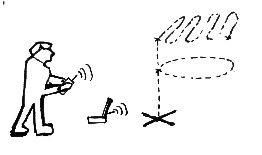
\includegraphics[width=4cm]{images/intro/outputonlinejpgtools.jpg}
%   \caption{An environment for outdoor deployments.}
%   \label{fig:outdoors}
% \end{marginfigure}


A carrier drone is developed to simplifying the integration of new sensors in preparation for outdoor operation. An unmanned aerial vehicle system has two parts, the drone itself and the control system. The design elements examined here are the following:
\begin{itemize}
    \item \textbf{Drone Components}: onboard sensors and navigational systems for stable, semi-autonomous flight.
    \item \textbf{Control system}: Flight system features like piloting modes and datalinks that are specific to the types of operation.
    \item \textbf{Navigation parameters}: safeguards and automated parameters to provide safe and secure flight.
\end{itemize}

\begin{marginfigure}%[!h]
    \raggedright
    
    % 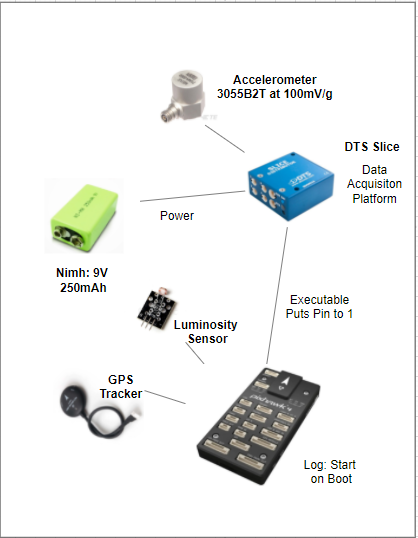
\includegraphics[height=7cm]{images/stage_system/slice_arch.PNG}
    % 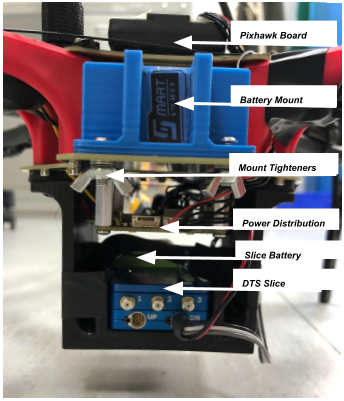
\includegraphics[height=7cm]{images/stage_system/payload_installed.png}
    \hspace{0.25cm}
    \vspace{1cm}
    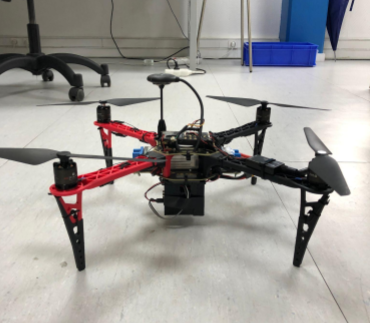
\includegraphics[width=4cm]{images/stage_system/drone_setup.png}
    \caption{Final Drone Setup}
    \label{fig:drone_presentation}
\end{marginfigure}


\begin{figure*}[!h]
    \raggedright
    \hspace{1.5cm}
    {\includegraphics[width=7.5cm]{images/stage_system/drone_setup/carrier_drone.png}}
    
    \caption{Carrier Drone Design and Flight Environment.}
    \label{fig:RC_screen}
\end{figure*}


This sections examines the flight-related functionality, including piloting features, navigation safeguards and other automation tools. Sections \ref{section:environment} and \ref{section:vibrations} document the design of two modular payloads for collecting Atmospheric Data and Vibration Data.

%     \item Simplifying the procedures to reconfigure the board for new flights.
%     \item Safeguard highly sensitive equipment to parasitic vibrations.
%     \item Overall robustness to shocks.
% \end{itemize}



\subsection{Onboard Components}\label{section:msp_overview}

The body of an unmanned aerial vehicle is designed for propulsion, via electrical motors and their associated navigation system. This is where all the sensors and navigational systems are present.

% \subsection{Hardware}
% Three key elements are examined: the drone frame and two methods for data acquisition. 
% Further hardware (system setups and sensor choices) are included in further chapters.

\subsubsection{Drone Frame and Power Distribution}

\begin{marginfigure}%
  \hspace{0.25cm}
  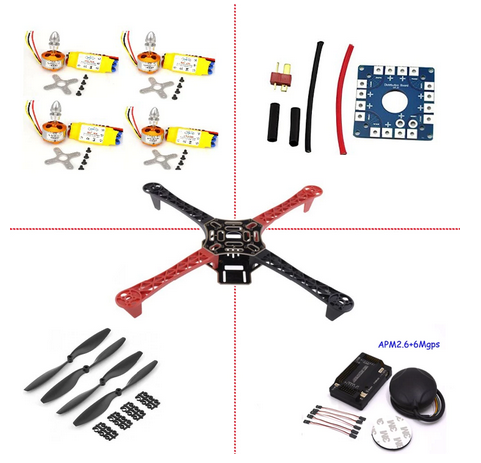
\includegraphics[width=4cm]{images/stage_system/f450_setup.png}
  \caption{ The F450 drone, along with (clockwise from top) a Power Distribution Board, a GPS setup, propellers and motor-ESC pairs.}
\end{marginfigure}

The UAV chosen for this system is the DJI's F450 Flame Wheel frame, a self-assembled platform designed for aerial photography and entertainment purposes.  This quadrotor is common in research as it provides the space required to assemble new modules \cite{sørensen_jacobsen_hansen_2017} \cite{tezza_andujar_2019}.

The F450 is comparatively larger than many other drones; however, it is built of light-weight stiff carbon fibre and the battery and GPS can be stored away. It has an approximately 40 minute hover time without a payload and 20 minutes with maximum payload (3kg). 


\subsubsection{Flight Autopilot Controller}

%Flight Autopilot Controller
\begin{marginfigure}%
  \hspace{1cm}
  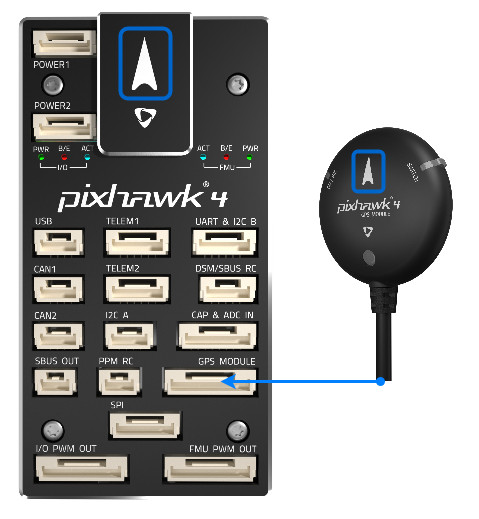
\includegraphics[width=3cm]{images/stage_system/pixhawk4_compass_gps.jpg}
  \caption{ The Pixhawk4 and GPS: an advanced autopilot adopted by academic and commercial developers \cite{px4_ecosystem}.}
\end{marginfigure}
The Flight Controller has inputs both from the Ground Station and the RC Controller. It acts upon the UAV Motors, logs data from the sensors and interacts with various payloads. Pixhawk \cite{px4_ecosystem} is an industry standard autopilot developed and jointly developed by 3DR Robotics and Ardupilot Group. Various robots such as RC cars, airplanes, and multicopters can be made, and firmware is provided for them using Pixhawk.  Motor control is achieved automatically, with enhanced stability to recover from wind surges. 


\subsubsection{Onboard Sensor Selection}\label{section:sensor_system}

\begin{marginfigure}%
  \vspace{1cm}
  
  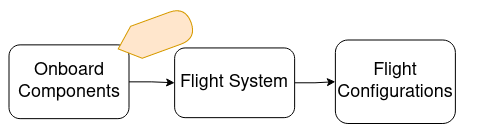
\includegraphics[width=5cm]{images/stage_system/drone_setup/components_order1.png}
  \caption{ Carrier Design, step 1.}
\end{marginfigure}
% \subsection{Overview of Sensor Systems}\label{section:sensor_system}

The carrier drone aims to simplify the integration of new sensors and associated data acquisition systems. To do this, a modular approach is adopted, whereas the setup is designed to simplify the board reconfiguration in new flights. 

Custom criteria are used to better understand the level of modularity for several sensor systems. 
\begin{itemize}
    \item \textbf{Large Field of View}: Whether said sensor requires a large field of view for optimal functioning,
    % \item \textbf{Requiring a Modular Setup}: a modular setup to simplify the board reconfiguration in new flights,
    \item \textbf{Vibration Sensitivity}: the vibration sensitivity of equipment in the case of parasitic vibrations. This element is desirable when carrying vibration-sensitive loads, for instance lidars, or items that might dismantle with vibrations. 
    \item \textbf{Independent Power Source}: an independent power source in the case of self-powered electronic circuits. 
\end{itemize}    

Table \ref{tab:payload_selection} looks at four possible sensor systems.

\begin{table*}[h]
  %\raggedright
  \footnotesize%
  \begin{flushleft}
    \begin{tabular}{lcccl}
      \toprule
      Criteria                      & Vibration  & Atmospheric & Rangefinder  & Camera \\
                                    & Data & Data & Data & Stream\\
      \midrule
      Independent Power Source      & \CIRCLE    &  \CIRCLE & \Circle & \Circle  \\
      Vibration Sensitivity         & \CIRCLE    &  \Circle & \CIRCLE & \CIRCLE  \\
      Large Field of View           & \Circle    &  \Circle & \CIRCLE & \CIRCLE \\
    %   Requires a Modular Setup      & \CIRCLE    &  \Circle & \CIRCLE & \CIRCLE\\
      \toprule
      
      Selection                     &  \ding{51} &  \ding{51} &  \ding{55} &  \ding{55} \\
      \bottomrule
    \end{tabular}
  \end{flushleft}
  \caption{Payload Selection Matrix.}
  \label{tab:payload_selection}
\end{table*}
% \CIRCLE \Circle \Circle \Circle \Circle

With a fully independent power source and less importance on the field of view, two sources of data are examined in more depth: the Vibration Data Subsystem and the Atmospheric Data Subsystem. The two DAQ systems are designed as independent subsystems.

% The two systems are fully designed and tested through two separate sections: the semi-autonomous scan of a zone (Section 2.4)


\subsubsection{DAQ Onboard Setup}\label{section:daq_modes}

\begin{marginfigure}%[!h]
    \raggedright
    \hspace{0.25cm}
    %\vspace{2cm}
    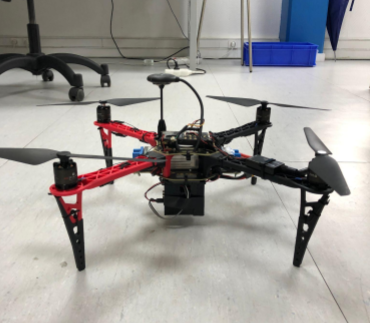
\includegraphics[width=4cm]{images/stage_system/drone_setup.png}
    \caption{DAQ Installation}
    \label{fig:fitting_payload}
\end{marginfigure}

A payload box can be used to encapsulate these subsystems, such that each module can be installed and removed during on-site drone reconfiguration. In the next section, a rectangular box is designed and 3d printed to attach upon the UAV. This box is designed for a variety of payloads. It is screwed on and can be removed easily, making it highly modular.

% \subsection{A multi-sensor payload}\label{section:msp_payload}


\begin{figure*}[h]
    \raggedright
    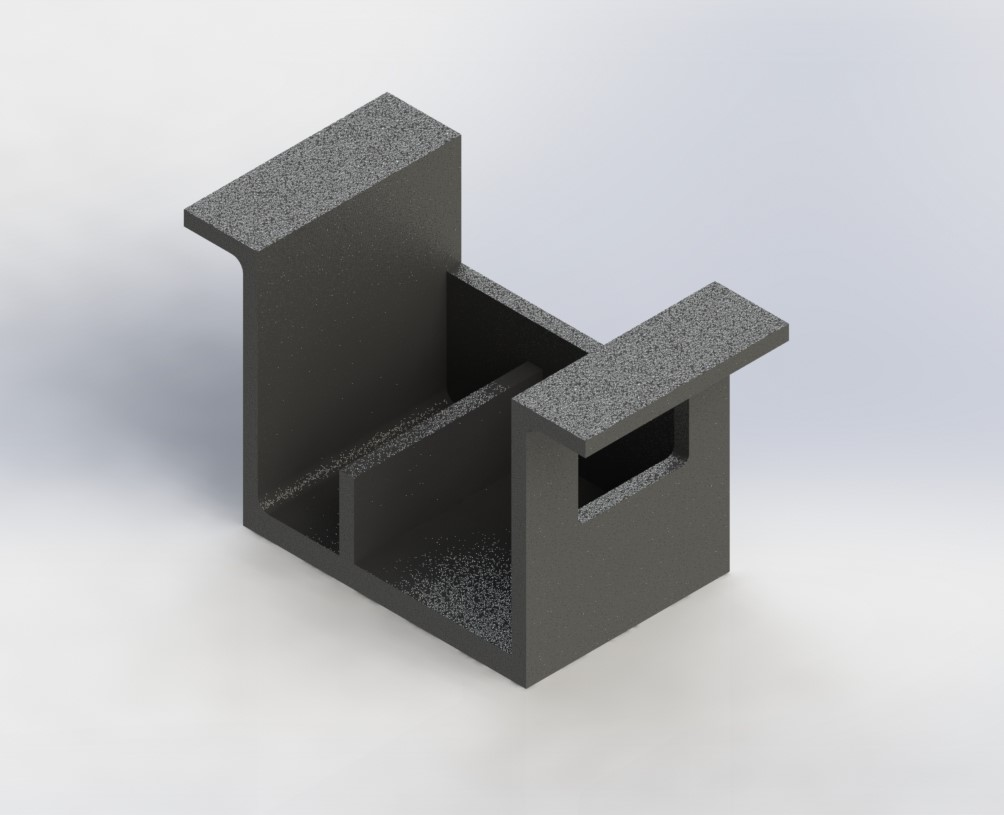
\includegraphics[height=2cm]{images/stage_system/renders/payload_box/1.JPG}
    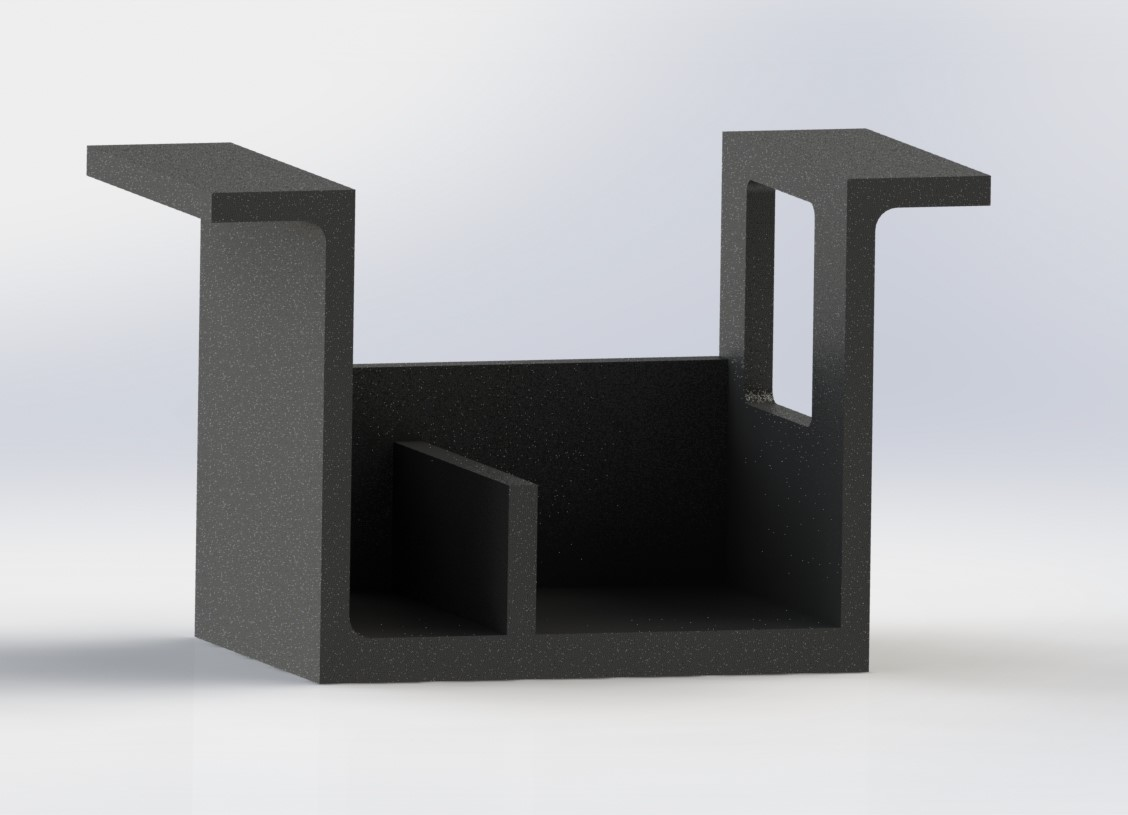
\includegraphics[height=2cm]{images/stage_system/renders/payload_box/2.JPG}
    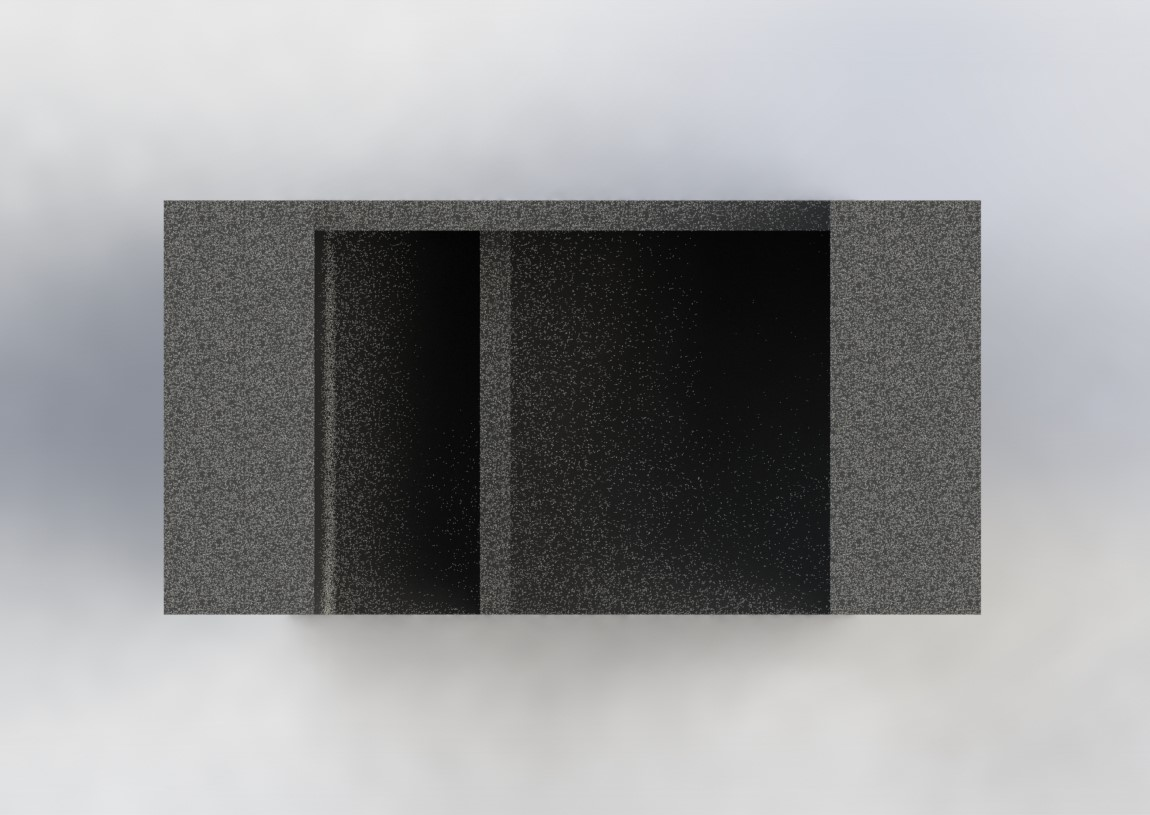
\includegraphics[height=2cm]{images/stage_system/renders/payload_box/3.JPG}    
    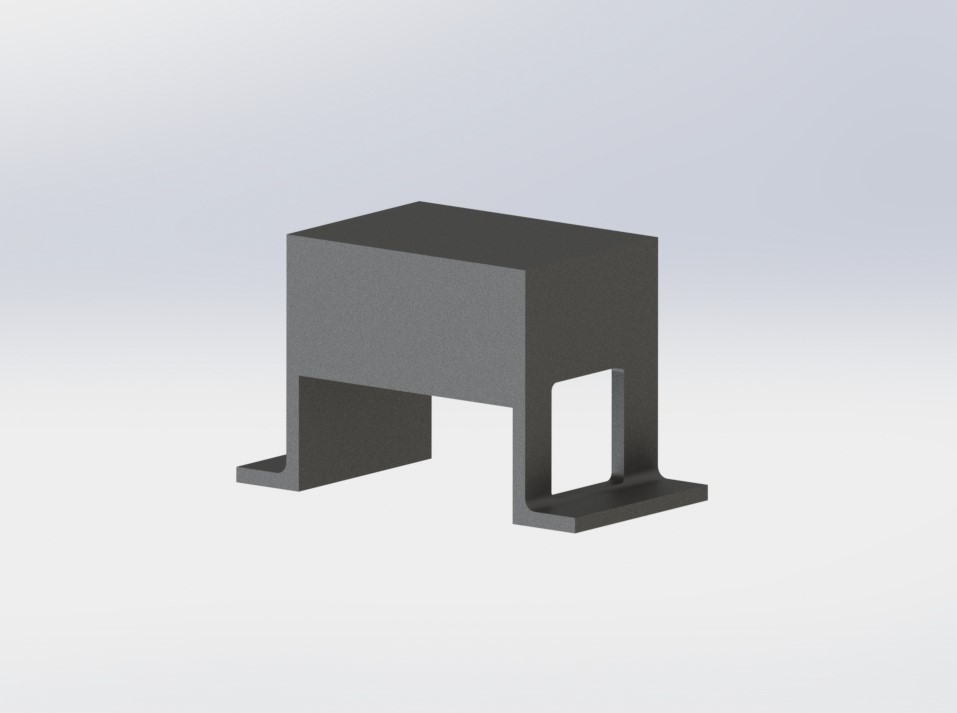
\includegraphics[height=2cm]{images/stage_system/renders/payload_box/4.JPG}
    \caption{Renders of payload box.}
\end{figure*}

The payload box offers an open window for cabling, as well as interstitial walls for the battery and the slice module. Using this design, the DTS Slice is installed on the UAV,  with a Battery as an energy source. The end result fits neatly on the drone (Figure \ref{fig:fitting_payload}). 


\subsection{Flight System}\label{section:flight_system}

The software controlling the UAV is a combination of elements. The flight system consists of a drone and all its associated components, for navigation, for the mounting of sensors, and for the logging the collected data. Figure \ref{fig:drone_presentation} presents the final drone configuration.

The flight system consists of a drone and all its associated components, for navigation, for the mounting of sensors, and for the logging the collected data. Figure \ref{fig:drone_presentation} presents the final drone configuration.

\begin{figure*}[h]
    \raggedright
    \includegraphics[width=11cm, left]{images/stage_system/drone_components.png}
    \caption{Expanded View of the UAV Ecosystem}
    \label{fig:msp_system}
\end{figure*}

The data acquisition systems seen here (DTS Slice and Arduino Nano) are expanded upon in Sections \ref{section:environment} and \ref{section:vibrations}.

\begin{marginfigure}%
  \vspace{1cm}
  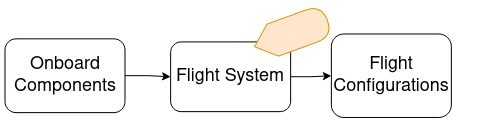
\includegraphics[width=5cm]{images/stage_system/drone_setup/components_order2.png}
  \caption{ Carrier Design, step 2.}
\end{marginfigure}


\subsubsection{UAV Flight Stack}


We chose to use the open-source PX4 flight stack \cite{px4_ecosystem} on the Pixhawk, running on top of the Nuttx real-time operating system. It has a number of mission critical features that are favorable for our research requirements. PX4 has a large research-oriented community of open-source practitioners, and tools for programming custom applications. 
% This function is implemented from our remote controller interface.

\begin{marginfigure}%
  \vspace{2cm}\hspace{0.3cm}
  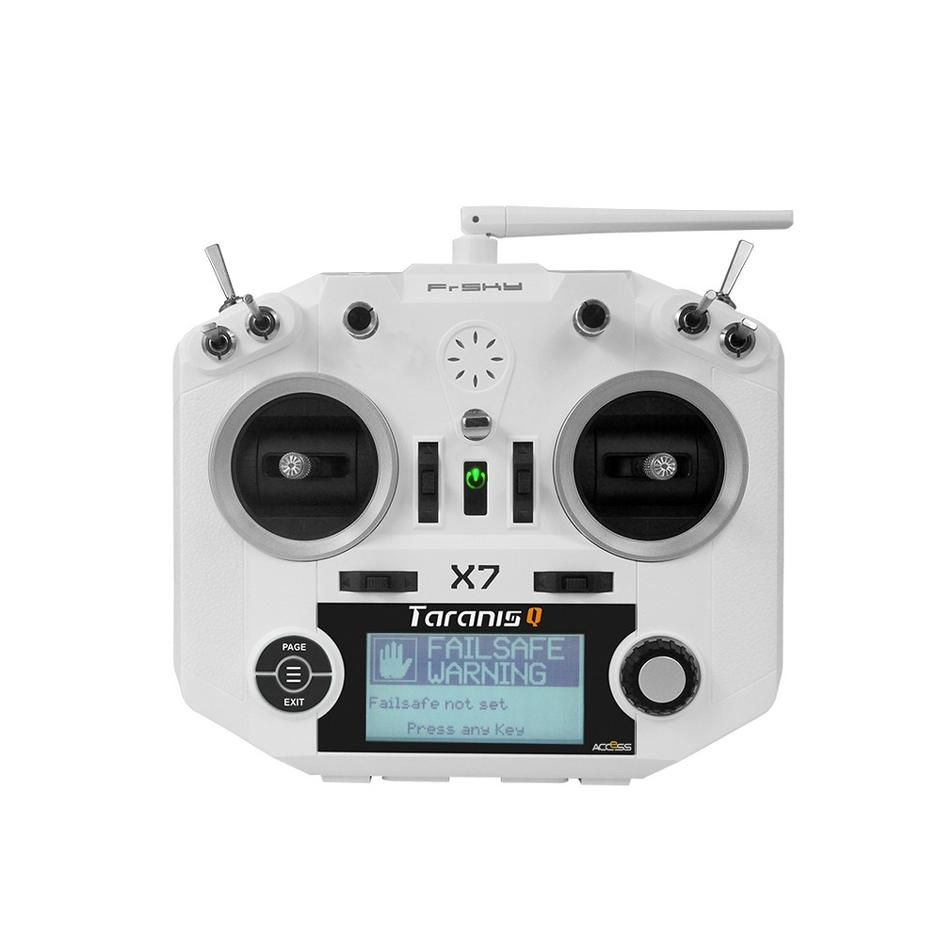
\includegraphics[width=4cm]{images/stage_system/taranis.jpg}
  \caption{ The Taranis X7 Remote Control: a reprogrammable remote for RC flight \cite{frsky_docs}.}
\end{marginfigure}

\subsubsection{Remote Controller and Datalink}

The Taranis is a common drone flight RC controller \cite{px4_docs}. It features 24 channels with a rapid baud rate and low latency, thanks to its high-speed module digital interface. The Q X7 transmits in the 2.4GHz range provides a secure and reliable link. 

The OpenTX firmware \cite{px4_docs} onboard the Remote Controller offers the possibility of assigning various switches to different flight modes, such as an arming mode in Figure \ref{fig:RC_screen}. Using two switches, we alternate between modes in the following order:

\begin{figure*}[!h]
    \raggedright
    \begin{minipage}{1.0\textwidth}
    \centering
    \hspace{0.5cm}\subfloat[1-1]{\hspace{-0.5cm} 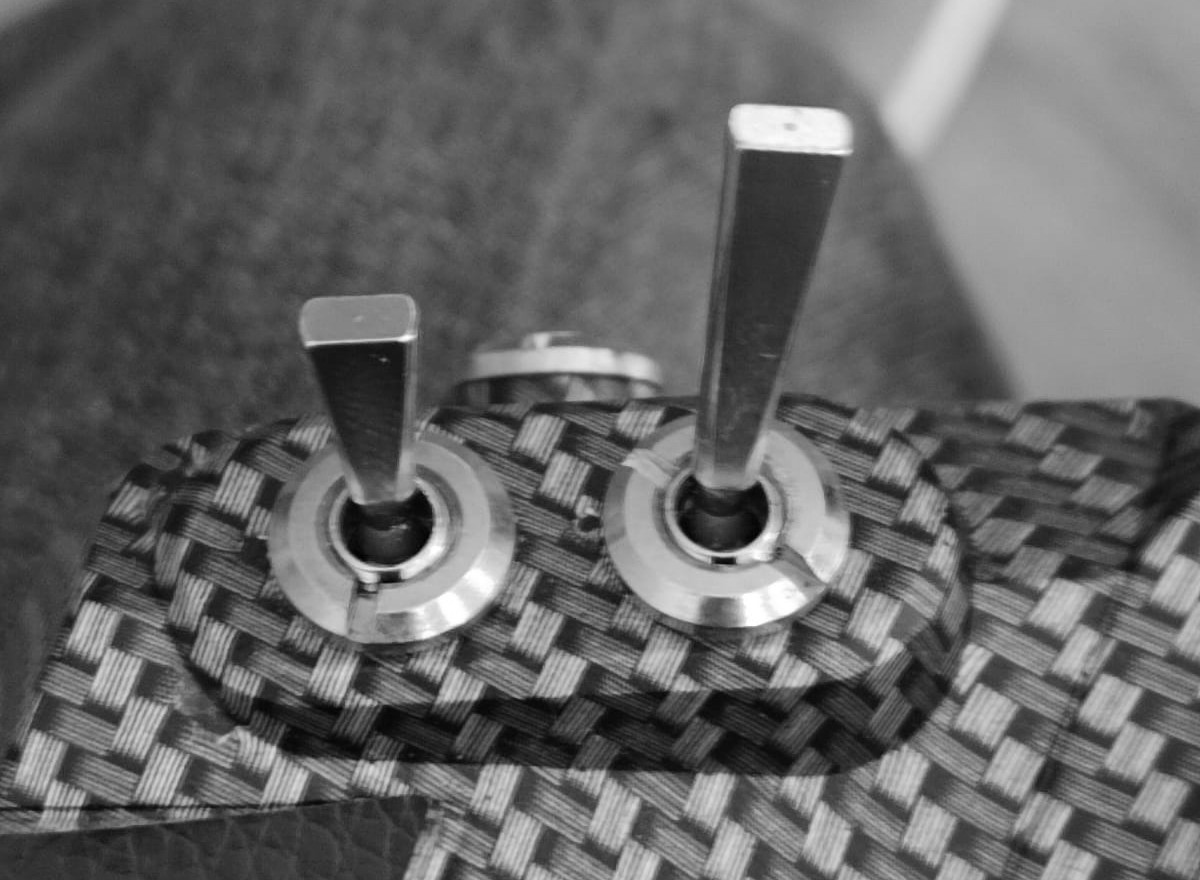
\includegraphics[width=2cm]{images/stage_system/switch_folder/1-1.jpg}}
    \hspace{0.5cm}\subfloat[2-1]{\hspace{-0.5cm} 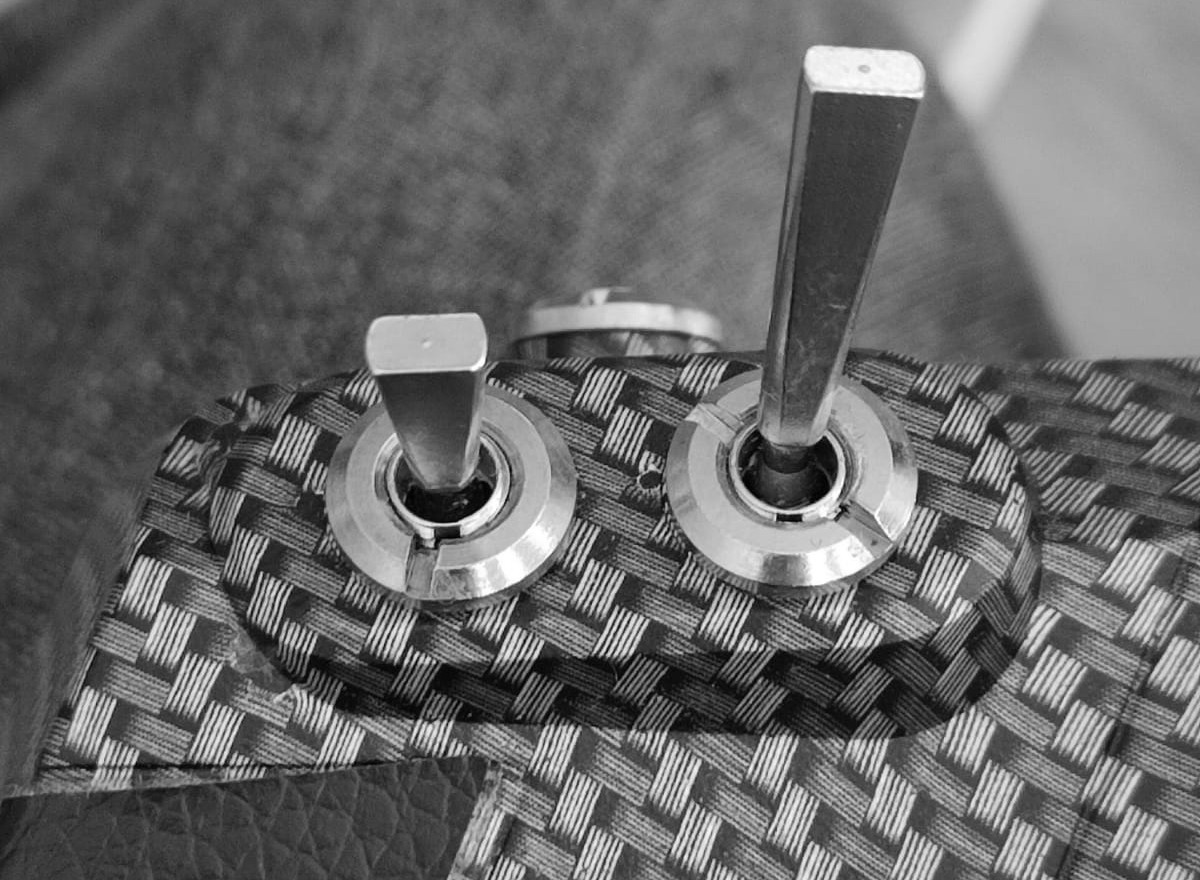
\includegraphics[width=2cm]{images/stage_system/switch_folder/2-1.jpg}}
    \hspace{0.5cm}\subfloat[3-1]{\hspace{-0.5cm} 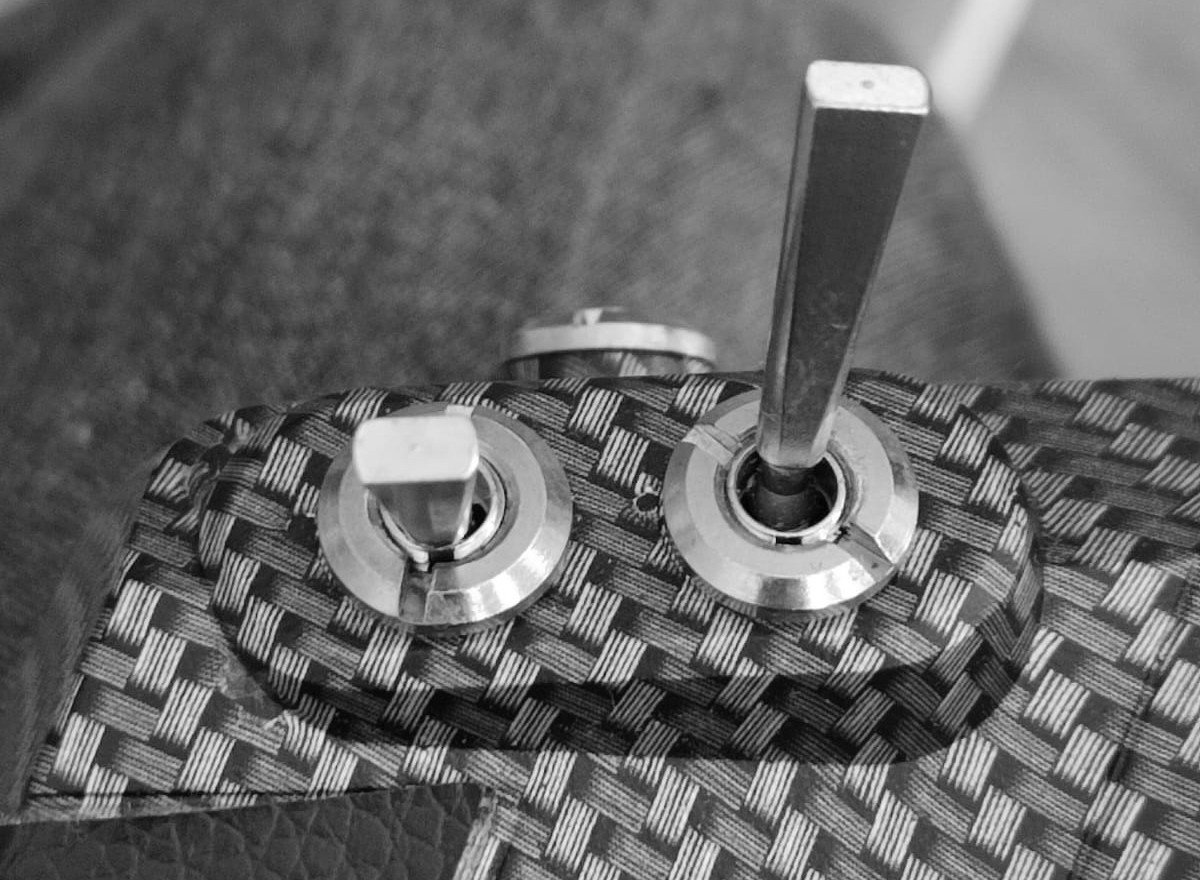
\includegraphics[width=2cm]{images/stage_system/switch_folder/3-1.jpg}}\\
    \hspace{0.5cm}\subfloat[3-2]{\hspace{-0.5cm} 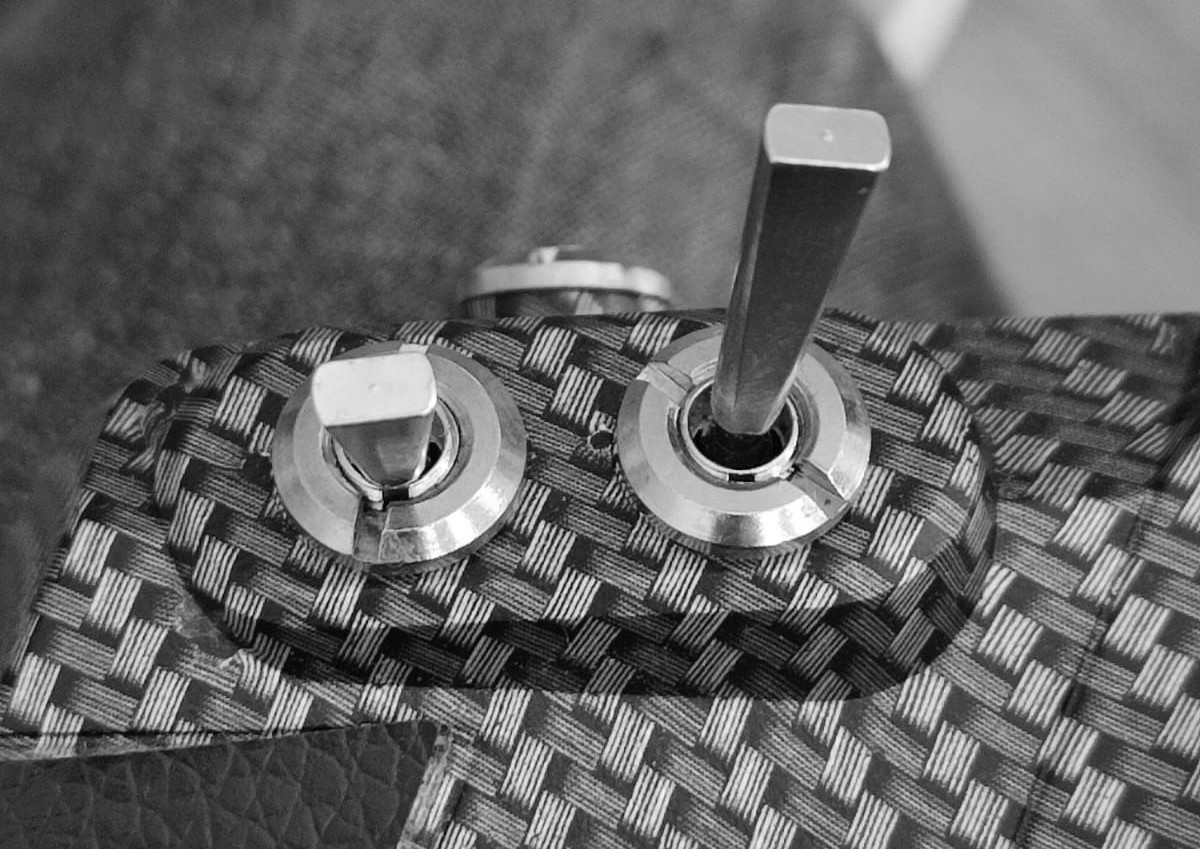
\includegraphics[width=2cm]{images/stage_system/switch_folder/3-2.jpg}}
    \hspace{0.5cm}\subfloat[2-2]{\hspace{-0.5cm} 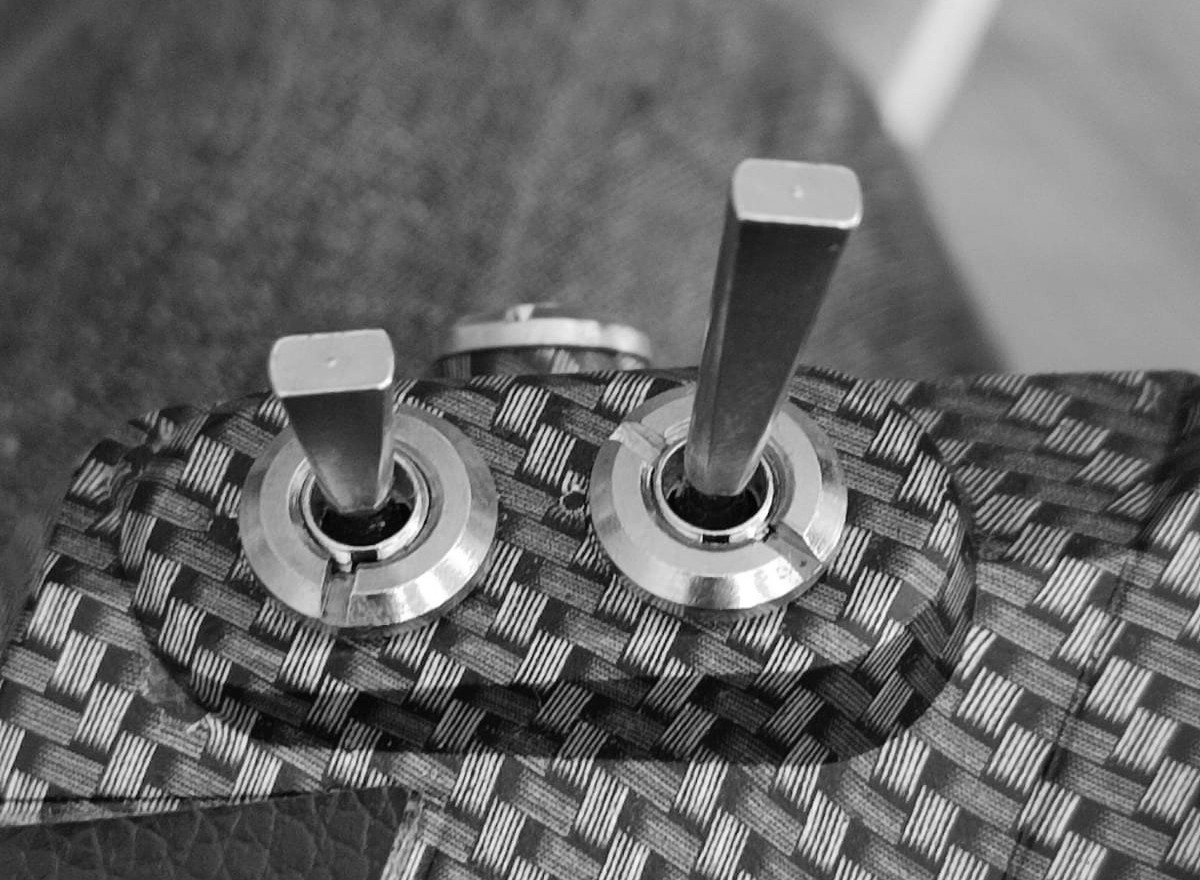
\includegraphics[width=2cm]{images/stage_system/switch_folder/2-2.jpg}}
    \hspace{0.5cm}\subfloat[1-2]{\hspace{-0.5cm} 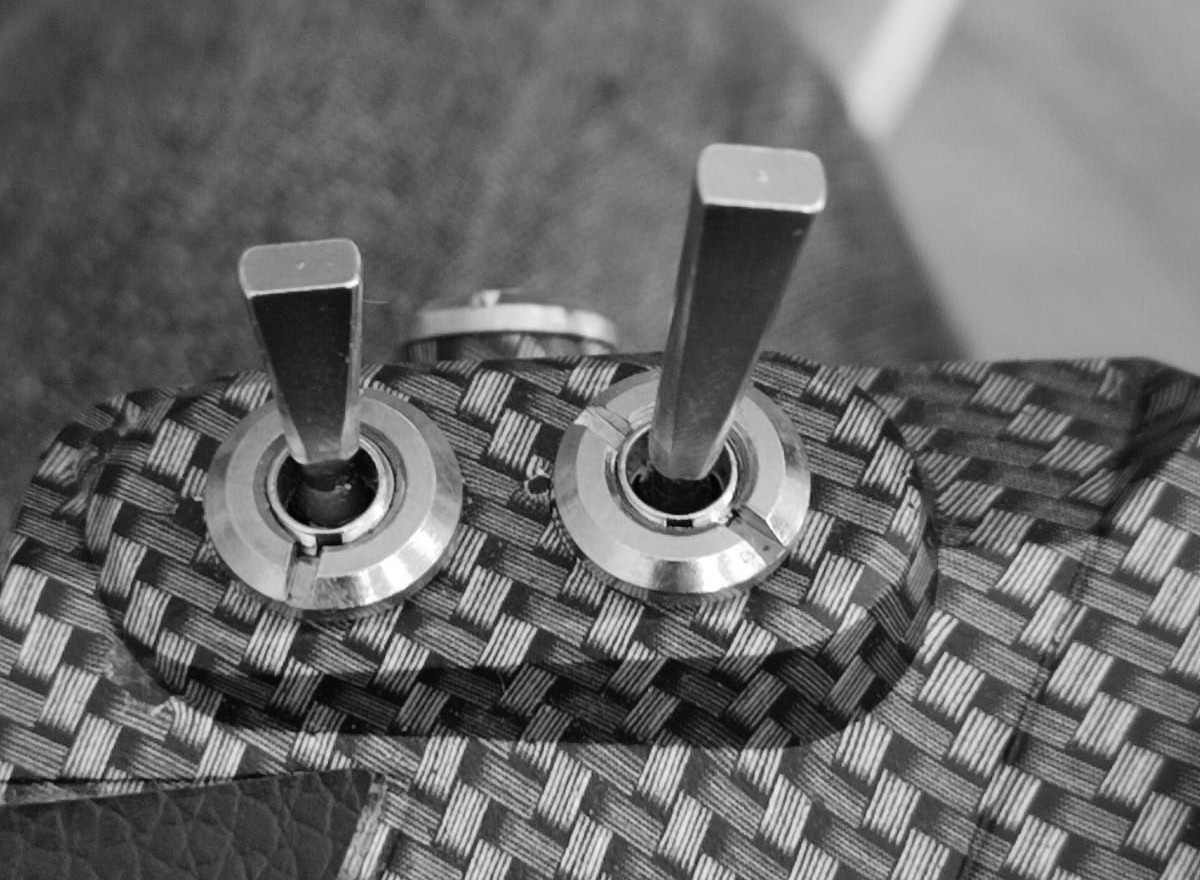
\includegraphics[width=2cm]{images/stage_system/switch_folder/1-2.jpg}}\\
    \hspace{0.5cm}\subfloat[1-3]{\hspace{-0.5cm} 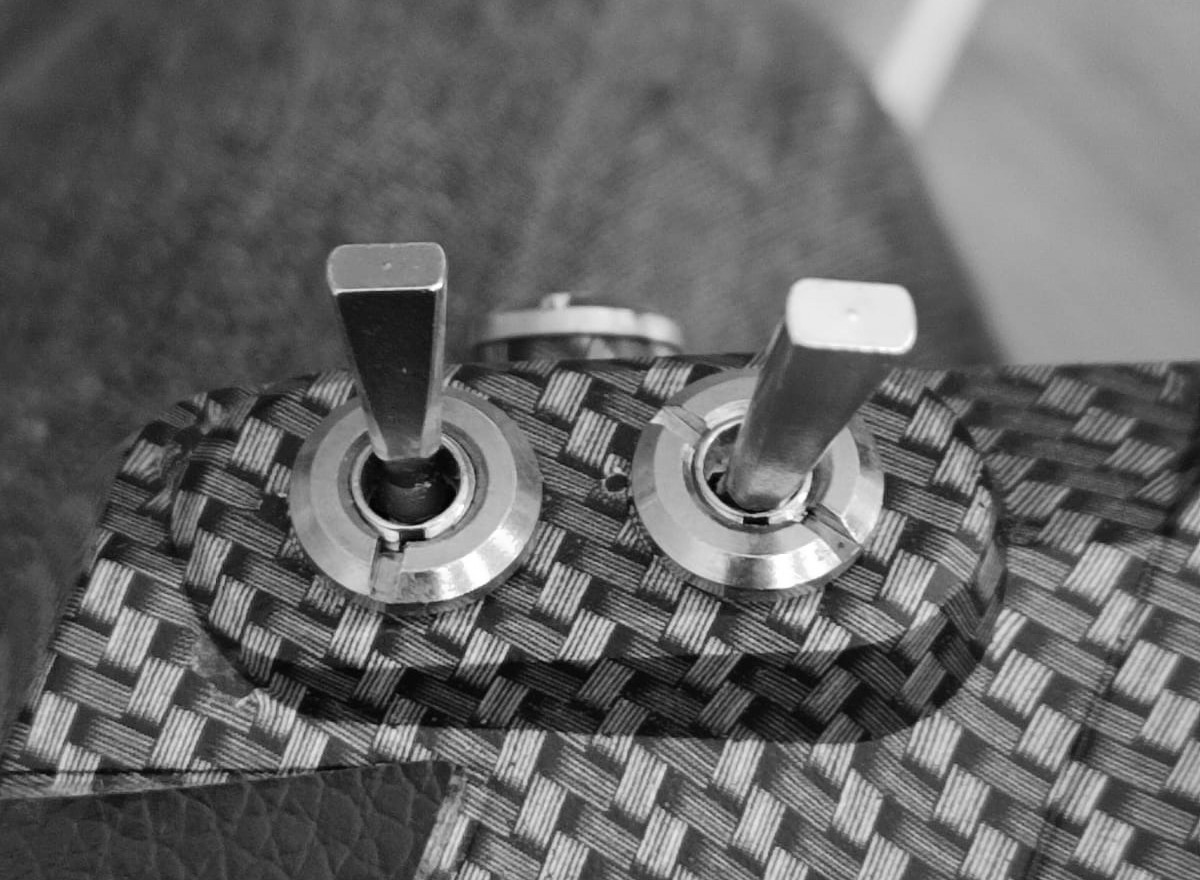
\includegraphics[width=2cm]{images/stage_system/switch_folder/1-3.jpg}}
    \hspace{0.5cm}\subfloat[2-3]{\hspace{-0.5cm} 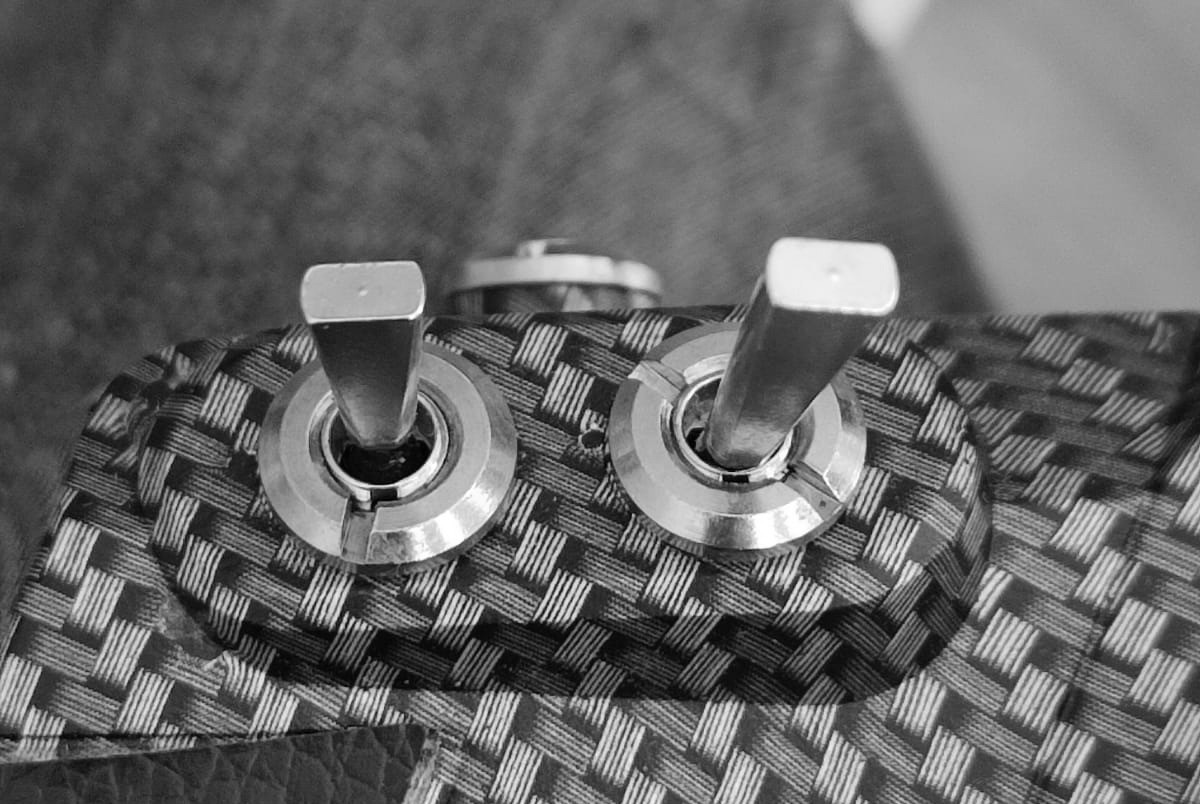
\includegraphics[width=2cm]{images/stage_system/switch_folder/2-3.jpg}}
    \hspace{0.5cm}\subfloat[3-3]{\hspace{-0.5cm} 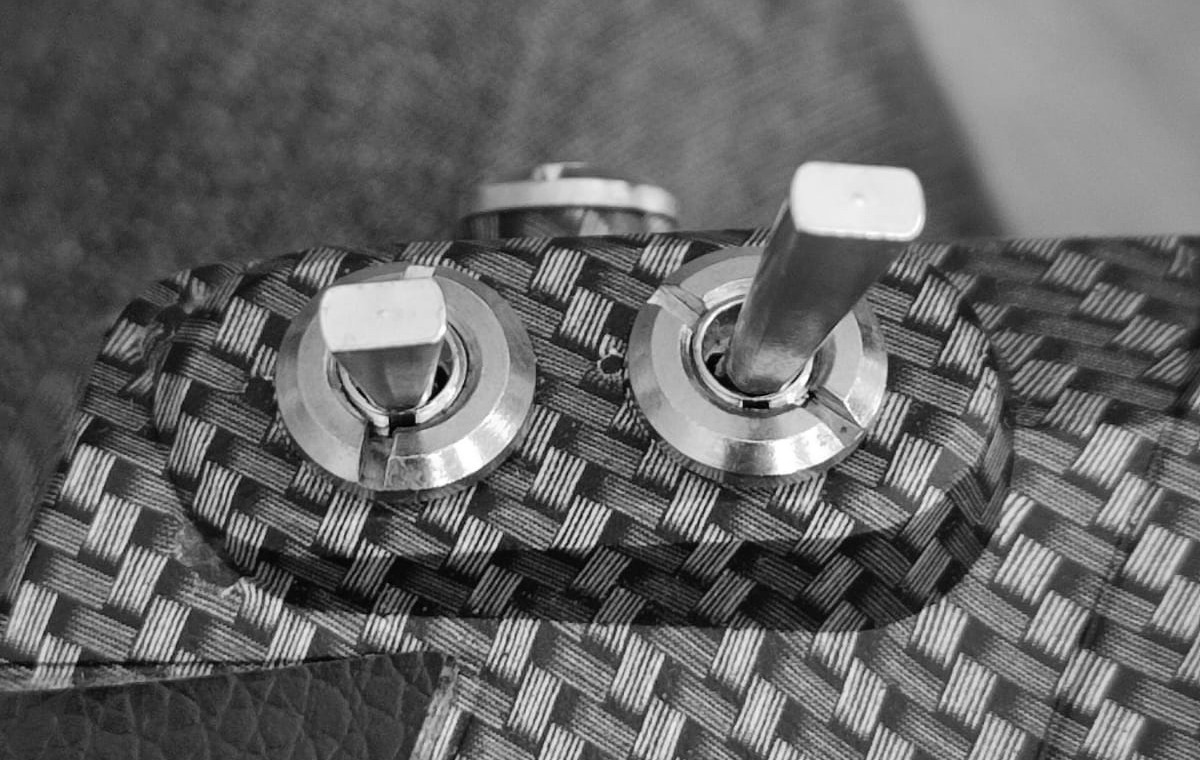
\includegraphics[width=2cm]{images/stage_system/switch_folder/3-3.jpg}}\\
    \end{minipage}
    \caption{Switch combinations and order of transitions.}
    \label{fig:switch_combinations}
\end{figure*}

\begin{marginfigure}%
  \vspace{0.3cm}
  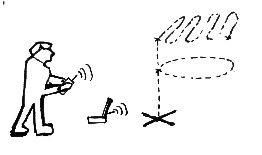
\includegraphics[width=4cm]{images/intro/outputonlinejpgtools.jpg}
  \caption{An environment for outdoor deployments.}
  \label{fig:outdoors1}
\end{marginfigure}

Using this technique, there are 9 modes that can be assigned a functionality. In this way, the pilot is given access to automatic functions. These assignments are done in Section \ref{section:config}.

%\pagebreak
\subsubsection{Ground Control Station and Telemetry}

\begin{marginfigure}%
  \hspace{0.3cm}
  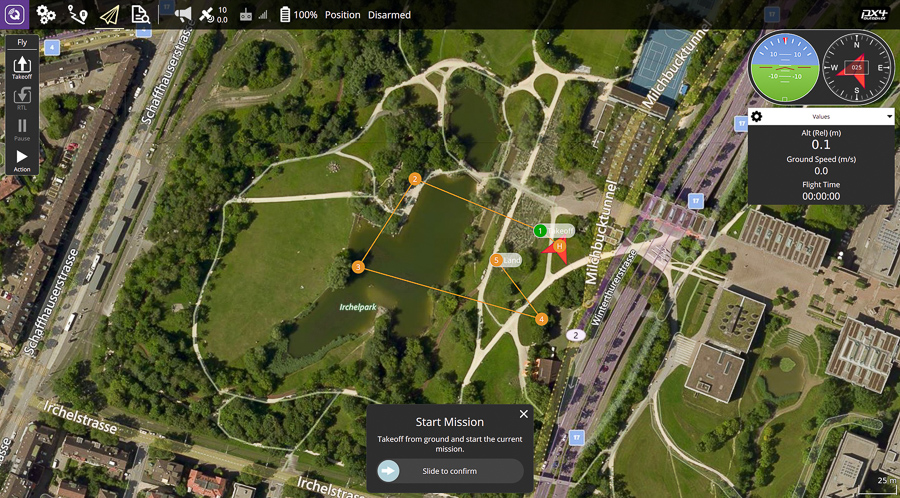
\includegraphics[width=4cm]{images/stage_system/qgc_presentation.jpg}
  \caption{ QGroundControl: an in-flight communication station \cite{px4_ecosystem}.}
\end{marginfigure}

Ground Control Stations (GCS) are sets of ground-based hardware and software that allow UAV operators to communicate with and control a drone and its payloads \cite{uav_components}. The QGroundControl ground control station \cite{px4_ecosystem} is used to communicate with the Pixhawk Autopilot via a Telemetry Radio. The communication is ensured by a Serial UART connection (MAVLink protocol \cite{px4_ecosystem}). 
% MAVLink is a light messaging protocol for onboard communication or components of drones. 
%This can be implemented in 14 languages, including C and C++, and various high-level APIs exist for the interaction between other systems such as drones and ROS. 

\begin{marginfigure}%
  \vspace{1cm}
  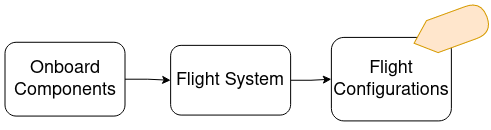
\includegraphics[width=5cm]{images/stage_system/drone_setup/components_order3.png}
  \caption{ Carrier Design, step 3.}
\end{marginfigure}

\subsection{Configurations for Flight Operation}\label{section:config}

Through the software outlined above, the drone can be remotely controlled or fly autonomously. Further mode configurations assist to program the drone for specific tasks. A flight setup is adopted here for the experiments in the next chapters, that is advantageous in terms of ease-of-use, programmability and safety.



\subsubsection{Pilot Configuration }\label{section:pilot_modes}

The switch is used to coordinate multiple flight modes. These modes are useful to alternate between very controlled motion, and smoother motion for data acquisition.

% \begin{table*}[h]
%   %\raggedright
%   \footnotesize%
%   \begin{flushleft}
%     \begin{tabular}{lccccl}
%       \toprule
%       Flight                       & Switch   & Roll and     & Yaw   & Throttle & Releasing \\
%       Modes                        &  Combination    & Pitch Sticks & Stick &          & Controls \\
%                                     % & Acceleration & Sensors & Sensor & System\\
%       \midrule
%       1. Position   & 1-1    &  Acceleration & Rate of    & Speed of       & Break, Level  \\
%                     &        &  over Ground  & rotation over      & Ascent and & and Lock   \\
%                     &        &               &  Horizontal     & Descent & at Point  \\                    \\
%       2. Altitude   & 1-2    &  Movement     & Rate of rotation  & Speed of         & Level and   \\
%                     &        &  over Ground  & over Horizontal   & Ascent-Descent   & Maintain  \\
%                     &        &               &                   &                  & Altitude  \\
%                     \\           
%       3. Stabilized & 1-3    &  Attitude    & Rate of rotation    & Altitude        & Center \\
%                     &        &  Angle       & over Horizontal     & and speed       & Deadzone \\
%                     % \\
%       \bottomrule
%     \end{tabular}
%   \end{flushleft}
%   \caption{Flight Mode Assignment for RC Controller.}
%   \label{tab:mode_description}
% \end{table*}

These three modes are configured to switches 1-1, 1-2 and 1-3. In a single flight operation, Position mode is used to position the drone at a hover, Altitude Mode is used to move on a horizontal plane, and Stabilized mode is used to move freely in 3D space.

% \pagebreak
% \subsubsection{Safety Features }\label{section:safety_modes}


% \begin{marginfigure}%[!h]
%     \raggedright
%     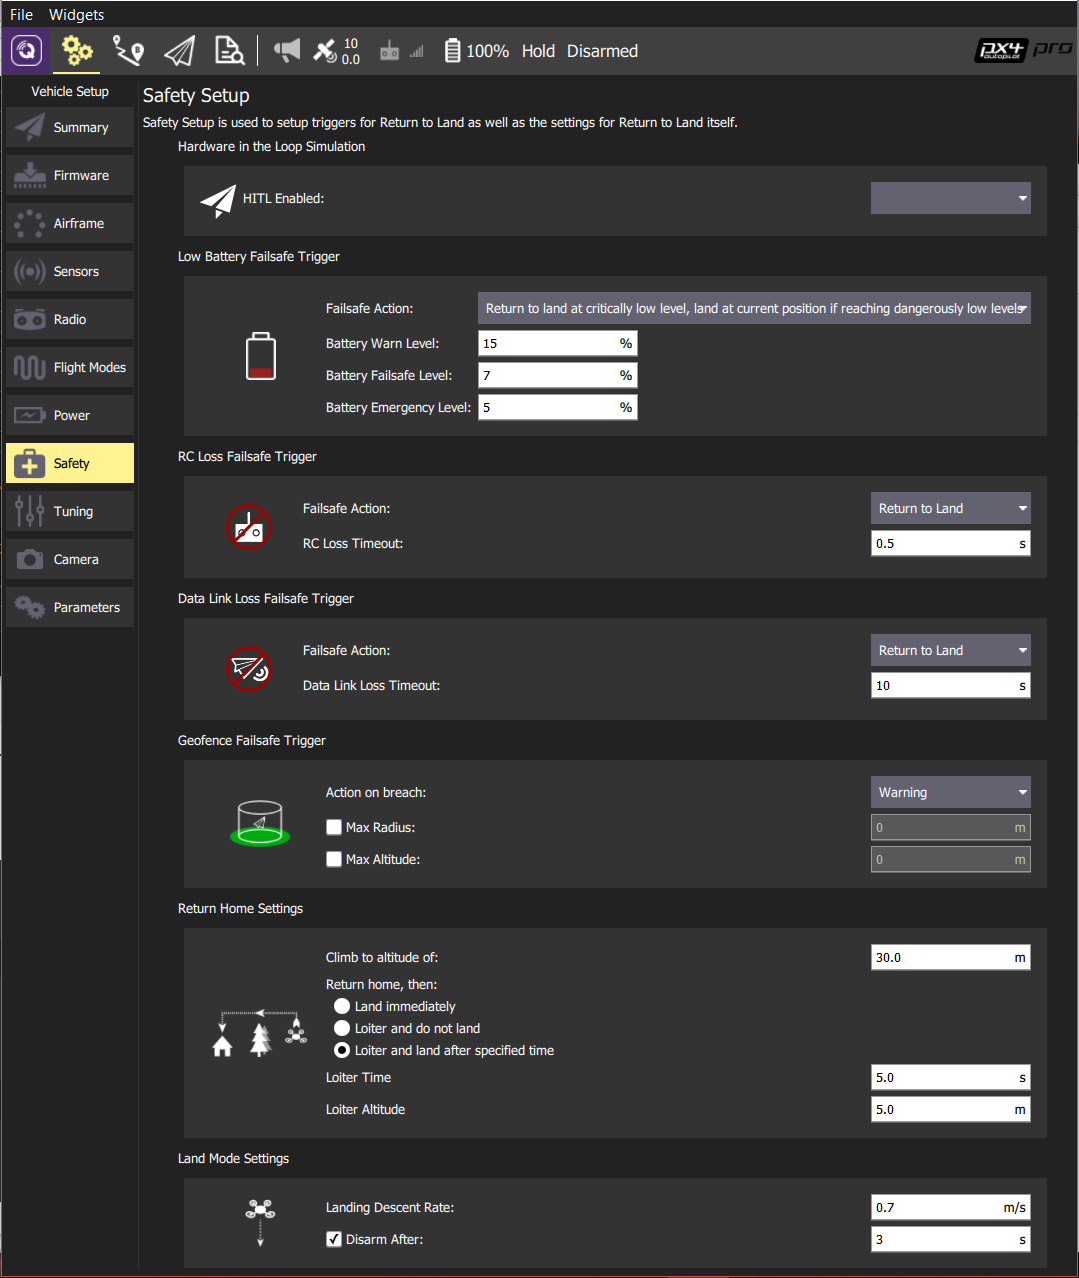
\includegraphics[width=5cm]{images/stage_system/drone_setup/PX4Safety.jpg}
%     \caption{Configuration of failsafes}
%     \label{fig:safety_features}
% \end{marginfigure}


% \begin{itemize}
% \item RC Loss: triggered if the RC transmitter link is lost in manual modes (by default RC loss does not trigger the failsafe in missions).
% \item  Geofence: "virtual" cylinder centered around the home position. If the vehicle moves outside the radius or above the altitude the specified Failsafe Action will trigger.
% \item Low Battery: triggered when the battery capacity drops below one (or more warning) level values.
% % \item RC Loss: triggered if the RC transmitter link is lost in manual modes (by default RC loss does not trigger the failsafe in missions).
% % \item Data Link Loss: triggered if a telemetry link (connection to ground station) is lost when flying a mission.
% \item Return is a common failsafe action that engages Return mode to return the vehicle to the home position.
% \end{itemize}


\pagebreak

\begin{marginfigure}%
  \vspace{1cm}
  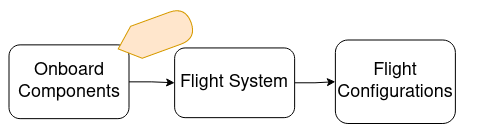
\includegraphics[width=5cm]{images/stage_system/drone_setup/components_order1.png}
  \caption{ Carrier Design, step 1.}
\end{marginfigure}


\subsection{Damping Optimisation Study}

The last criterion of the design process is the safety of payloads onboard the drone during flight. For this reason, the payload is required to be vibration-sensitive. 

The goal of this section is to minimize the vibrations experienced by the payload during flight. A damping test is carried out to determine the amount of damping material on the payload box. This procedure forms part of the drone design process determine an optimal damping volume.


\begin{marginfigure}%[!h]
    \raggedright
    \hspace{1cm} \subfloat[Wall Thickness]{\hspace{-0.8cm}\includegraphics[width=4cm]{images/stage_system/payload_thickness2.png}}\\
    \subfloat[AET vibration damping material]{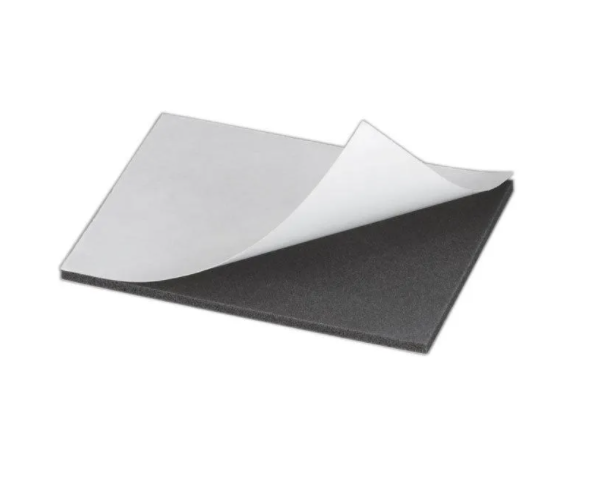
\includegraphics[width=5cm]{images/stage_graphs/aet_material.PNG}}
    \caption{Installation of Damping Material}
    \label{fig:aet}
\end{marginfigure}

\subsubsection{Hypothesis}
More shock absorption material leads to a smoother frequency response. 


\subsubsection{Prediction}


Two payloads A and B are attached to the drone. They vary by the amount of damping material (see Figure \ref{fig:aet}). The hypothesis is validated if payload A has better damping sensibility than payload B. The damping sensibility is associated to the Frequency Response of each payload. 

\subsubsection{Methodology}



\textit{Measurement Equipment Setup} \hspace{0.3cm} Our approach is a comparison of vibrations experienced by the drone payload during flight, compared to the vibrations on the drone frame. We do so by gathering acceleration data. For each flight, two accelerometers are used: a reference accelerometer on top of the drone serves as the control, as well as a payload accelerometer installed within the payload box (Figure \ref{fig:damping}). 

\begin{itemize}
    \item Payload A has 8 mm high absorbers.
    \item Payload B has 4 mm high absorbers.
\end{itemize}

AET material is used as shock absorbers in the payload attachment (Figure \ref{fig:aet}). It is fitted between the payload and the drone, and screwed tight. This is the only point of contact. 
% and determining the PSD graphs as a measure of intensity of the vibration signals, for each payload, and separate from the payload.

\begin{figure*}[!h]
    \raggedright
    %\hspace*{\fill}   % maximize separation between the subfigures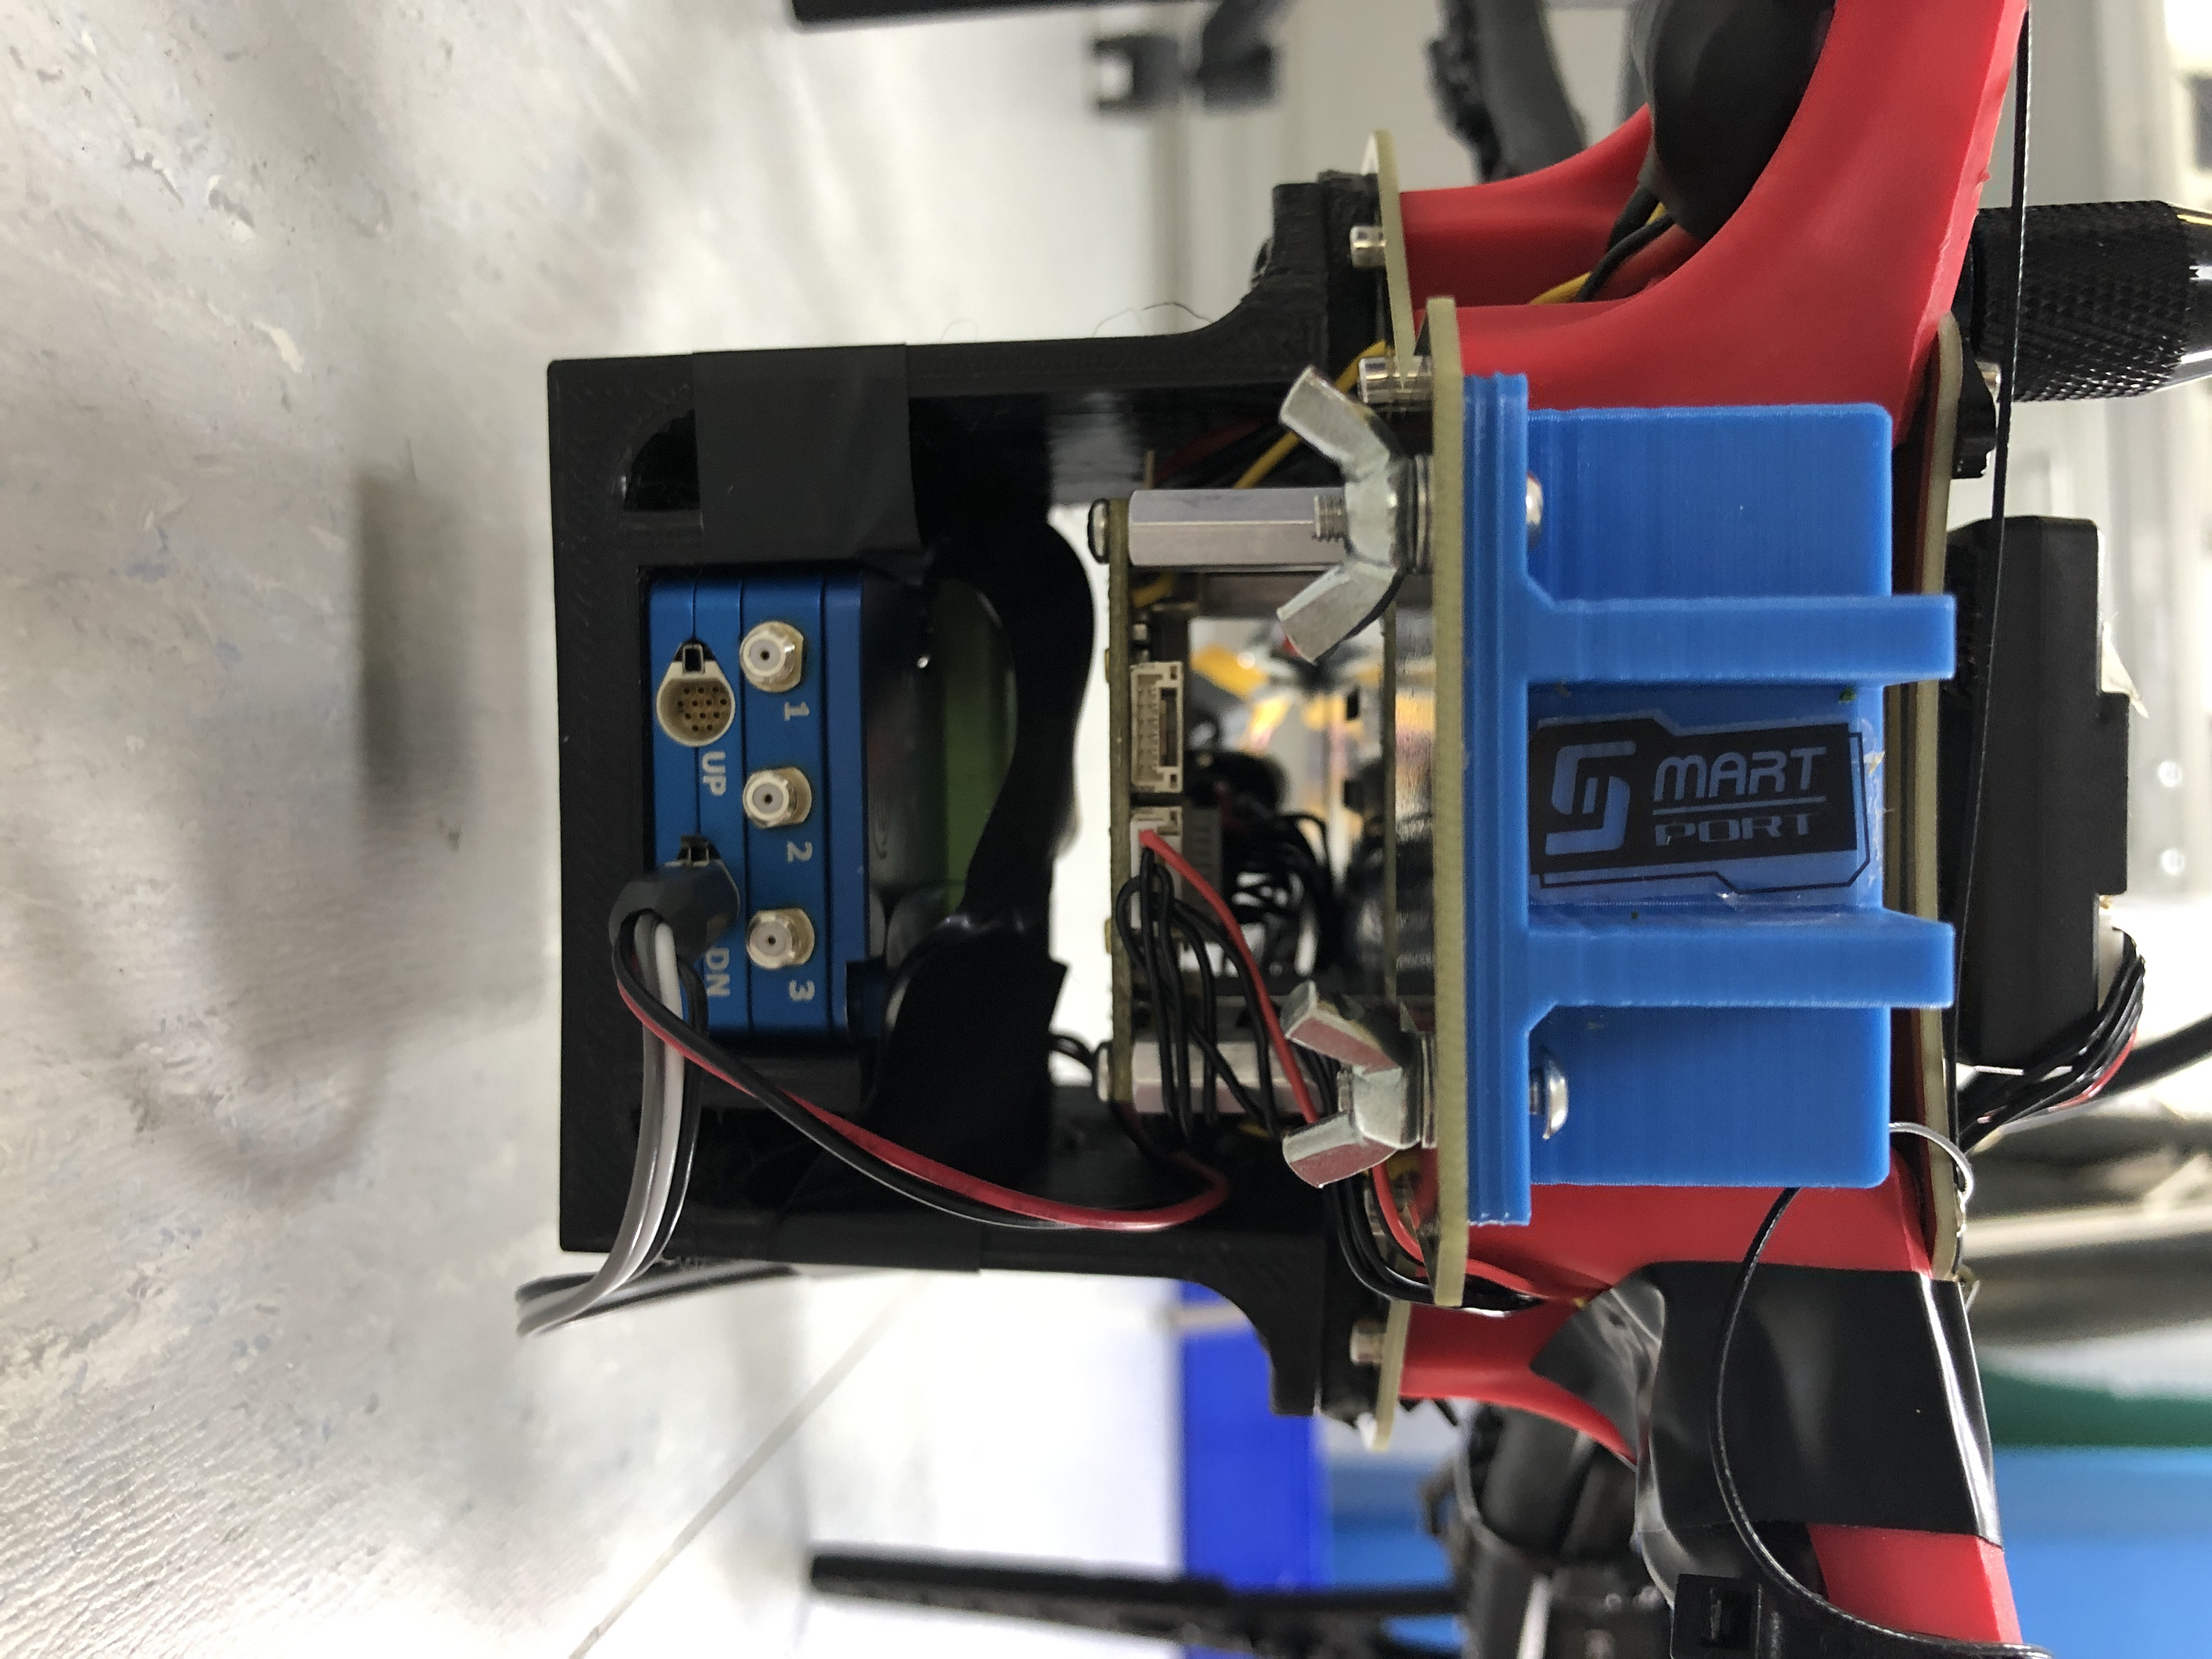
\includegraphics[width=4cm, angle=90]{images/stage_system/payload_onboard.JPG}
    % \subfloat[Shock absorbers are fitted between the payload and the drone, and screwed tight.]{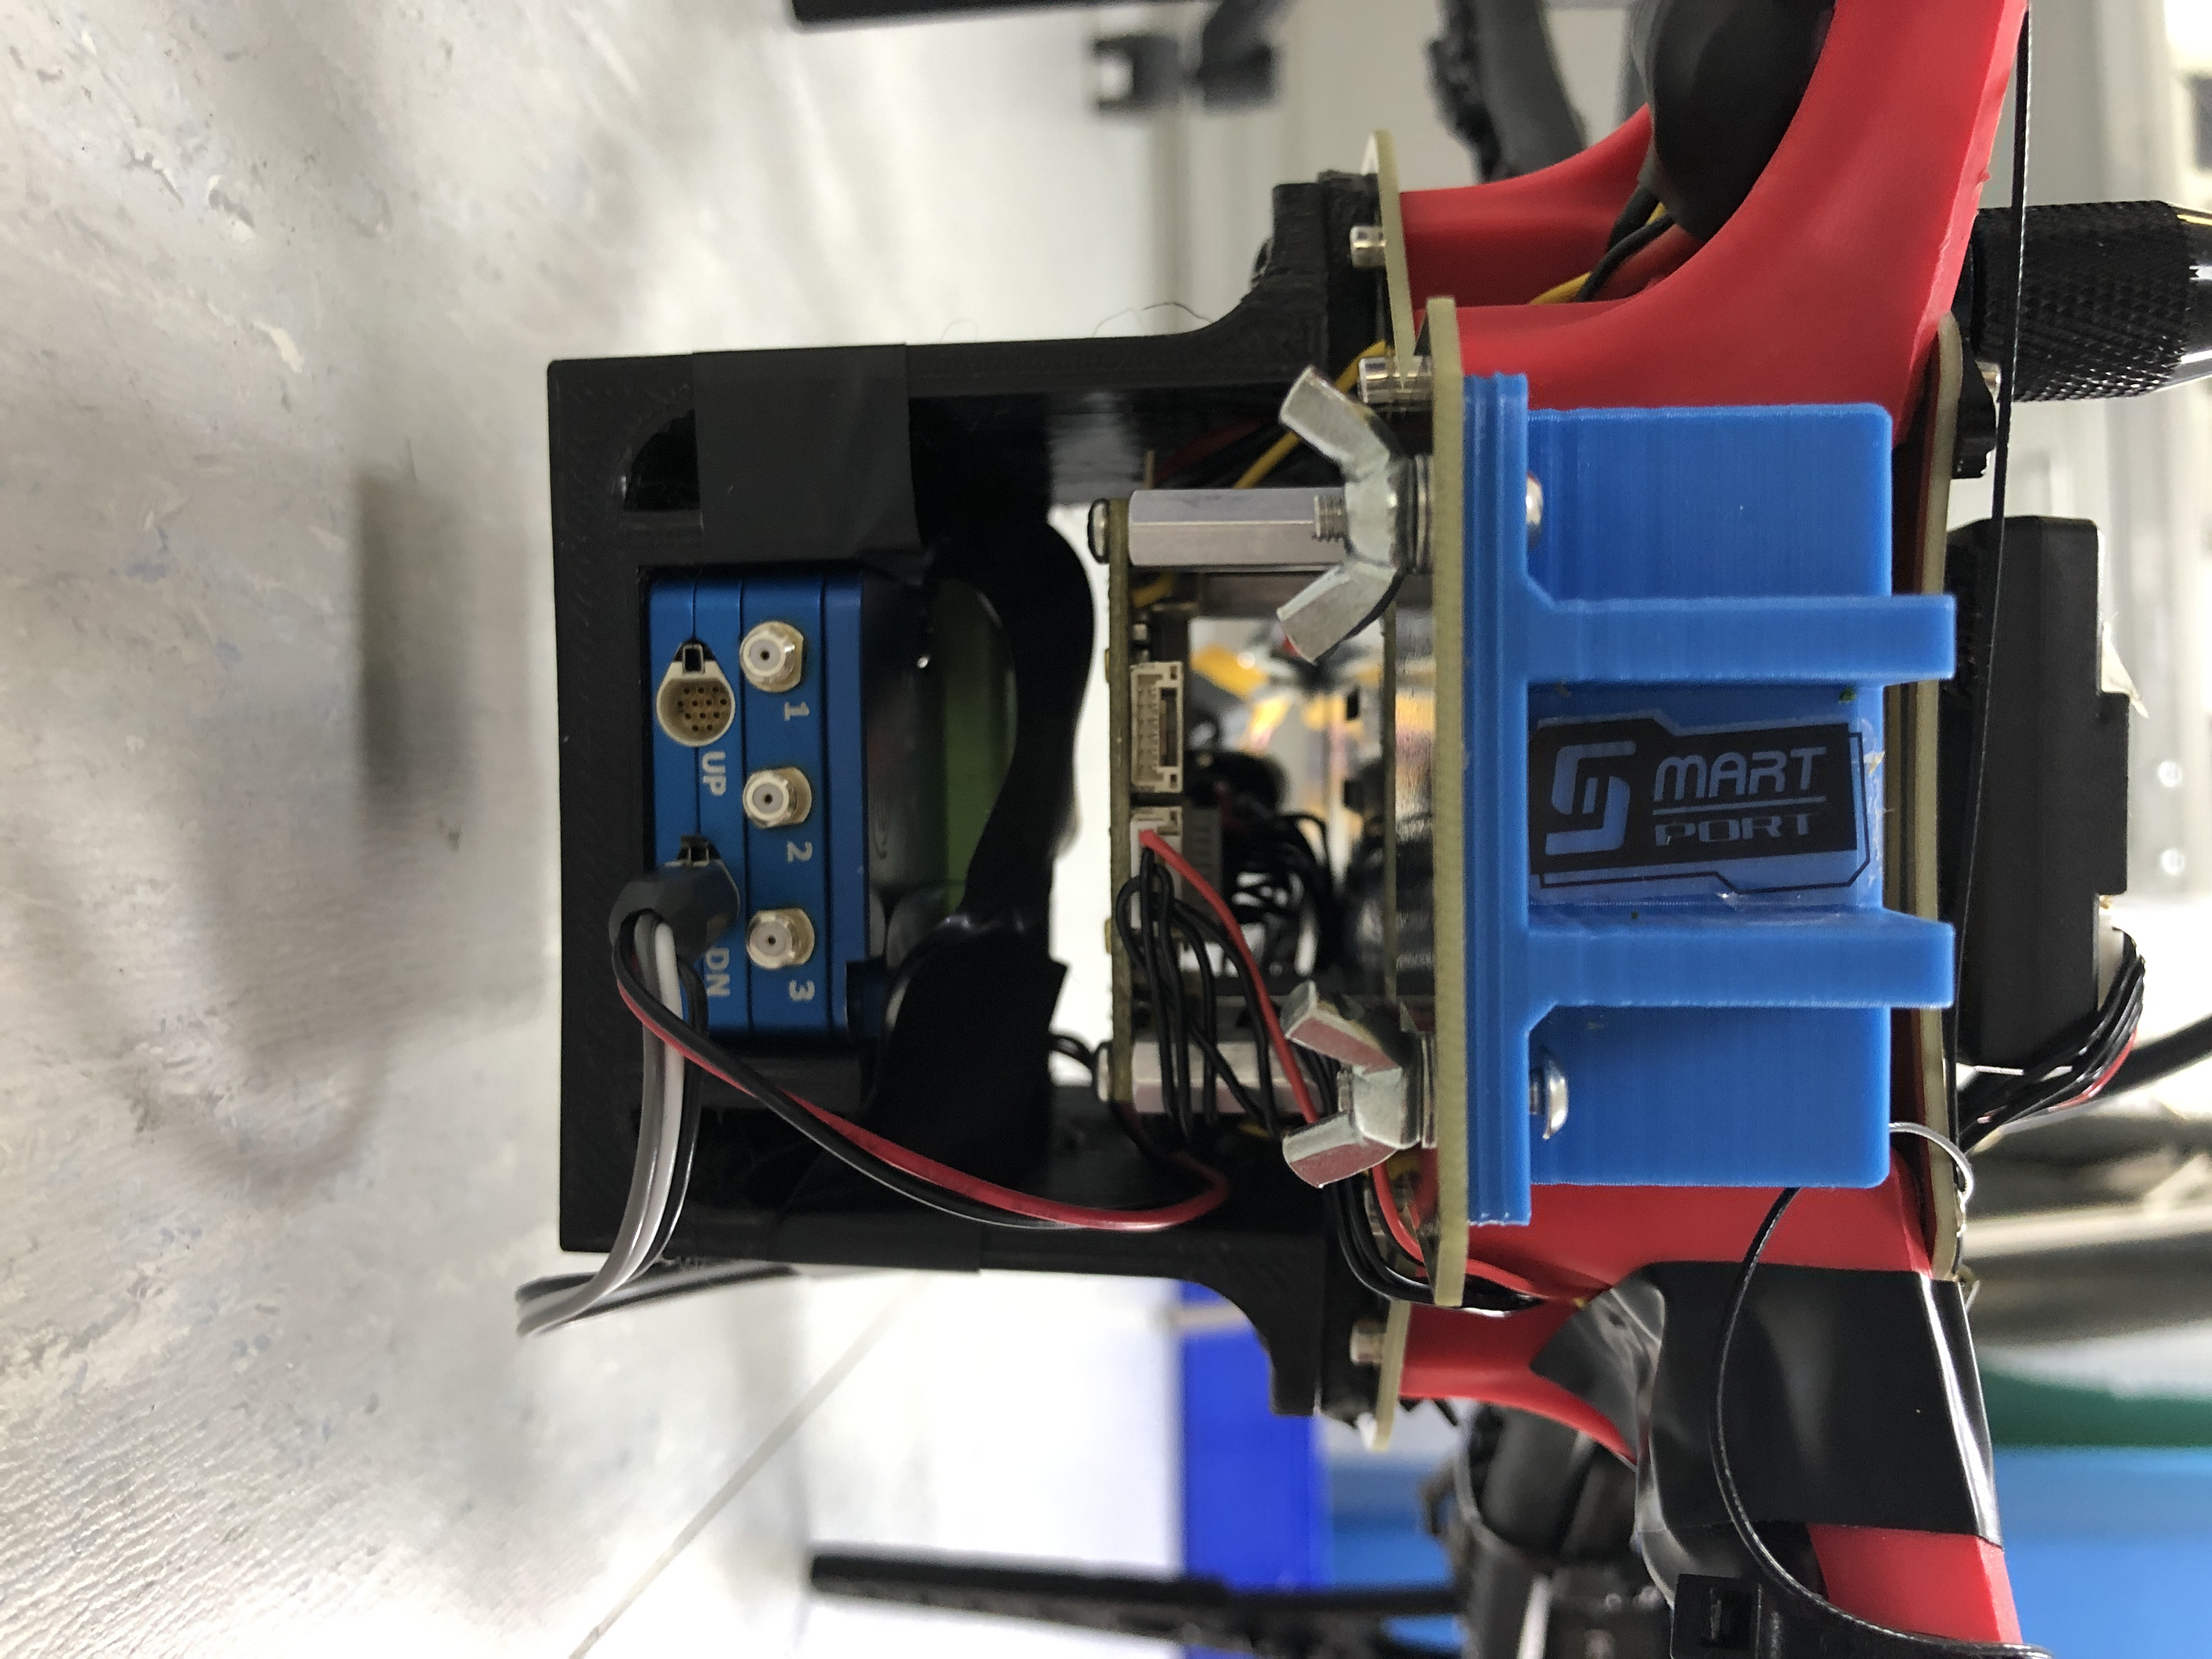
\includegraphics[height=4cm]{images/stage_system/payload_onboard.JPG}}
    %\subfloat[View of the two accelerometers]{
    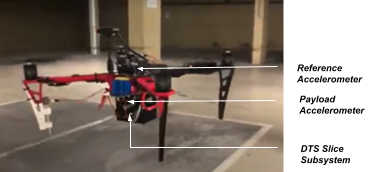
\includegraphics[height=5cm]{images/stage_system/absorption_test.png}
    %}
    \caption{View of the two accelerometers in Experiment setup}
    \label{fig:damping}
\end{figure*}

\begin{margintable}%[h]
  %\raggedright
  \footnotesize%
  \begin{flushleft}

    \begin{tabular}{lccl}
      \toprule
      Test Description &  \\%& Payload Accelerometer \\
      \midrule
      Test Date                     &  23/08/2021   \\%&  23/08/2021\\
      Test Time                     &  11:30:49     \\%&  11:30:49 \\
      %Test ID &   Flight3MOUSSE\_coupe \\%&   Flight3MOUSSE\_coupe \\
      Sample Rate                   &  25000 Hz \\%&  25000 Hz \\
      Hardware AA Filter            & 5000    \\%& 5000 \\
      Data Channels                 &	2       \\%&	2 \\
      Accelerometer Type            &	3055B2T       \\%&	2 \\
      %Channel Description           & 3055B2T\_REF \\%& 3055B2T\_Nacelle   \\
      Nb of Post-Zero Data Pts	& 750002	\\%& 750002  \\
      %Data Zero (CNTS)	            & 68	\\%& 33 \\
    %Scale Factor (EU/CNT)	        & 0.003781480491161	\\%& 0.003742169737816  \\
    %Scale Factor (mV/CNT)	        & 0.378148049116135	\\%& 0.374216973781586  \\
      \bottomrule
    \end{tabular}
  \end{flushleft}

  \caption{Parameters of the Payload Damping Test.}
  \label{tab:shock_absorption}
\end{margintable}

\textit{Acquisition Parameters} The DTS Slice is set up according to a few parameters. DAQ parameters are listed in Table \ref{tab:shock_absorption}. The DAQ was sampled at 25kHz. The anti-aliasing filter (AA), output scale factor and sampling rate are defined, among other factors.


\textit{Experiment Procedure} \hspace{0.3cm}  This experiment has two phases: in the first, Shock absorbers A are fitted; in the second, Shock absorbers B are fitted. This test proceeds in the following manner: 
\begin{enumerate}
    \item The drone is fitted with Payload A: a payload with a \textbf{greater} volume of shock absorber. See Figure \ref{fig:damping} as a reference.
    \item The drone is flown for 1 minute: forward, backward, to the left, and to the right. It is then landed.
    \item The drone is fitted with Payload B: a payload with a \textbf{smaller} volume of shock absorber.
    \item The experiment repeats.
\end{enumerate}

\textit{Post-processing} \hspace{0.3cm}  For each test, we calculate the PSD functions using the Welsh method, and calculate a ratio of the payload accelerometer's PSD over the reference accelerometer's PSD. This produces the Frequency Response Function.



% \begin{figure*}[h]
%     \raggedright
%     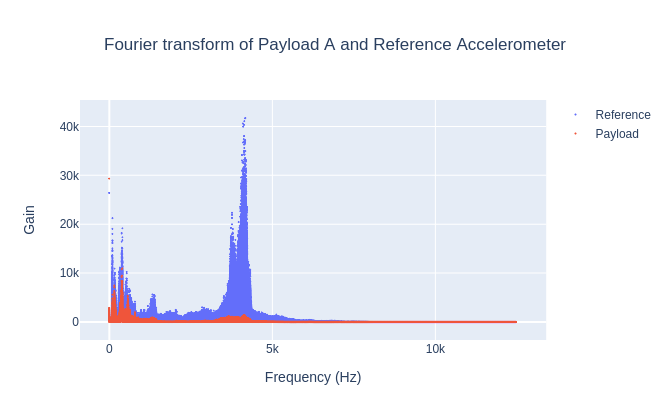
\includegraphics[width=6cm]{images/stage_system/design_graphs/fourier_transform.png}
%     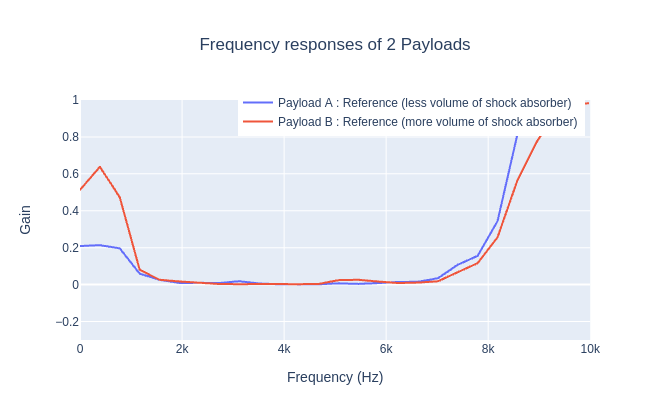
\includegraphics[width=6cm]{images/stage_system/design_graphs/freqresponse_payload.png}
%     \caption{Gain difference between the two payloads}
% \end{figure*}
\textit{Dataset} \hspace {0.3cm} The procedure was carried out on 23 August 2021 in an indoor parking space. The Google Drive experiment dataset \cite{vibrationmount_dataset} and a Youtube presentation video \cite{vibrationmount_video} are publicly available.
% Data processing is documented in the appendices \appendixcode{\ref{code:payload_damping}}.

%\pagebreak
\subsubsection{Results}
\textbf{PSD Plots} For each of the two payloads, we calculate the PSD functions using the Welsh method (Figure \ref{fig:PSD}).

\begin{figure*}[!h]
    \raggedright
    %\hspace*{\fill}   % maximize separation between the subfigures
    \subfloat[PSD Graph for  Payload A and Reference]{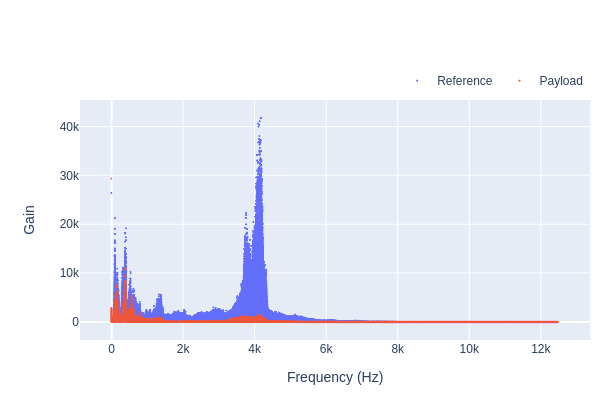
\includegraphics[height=4cm]{images/stage_system/design_graphs/PayloadA.png}}
    \subfloat[PSD Graph for Payload B and Reference]{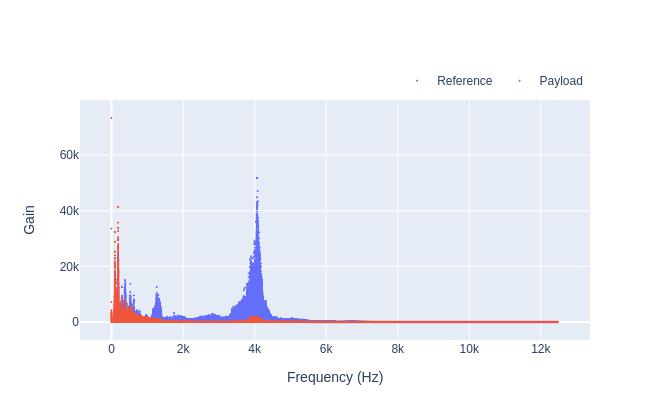
\includegraphics[height=4cm]{images/stage_system/design_graphs/PayloadB.png}}
    
    \caption{Development of the Gain Graphs to compare Payload A and B}
    \label{fig:PSD}
\end{figure*}

\textbf{Frequency Response Function} We calculate a ratio of the payload accelerometer's PSD over the reference accelerometer's PSD. This produces the Frequency Response Function (Figure \ref{fig:FRF}).

\begin{figure*}[!h]
    \raggedright
    %\hspace*{\fill}   % maximize separation between the subfigures
    {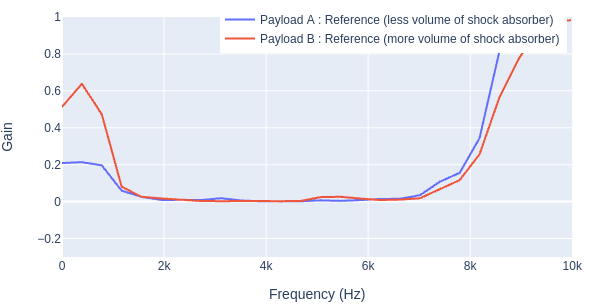
\includegraphics[height=5.5cm]{images/stage_system/design_graphs/freqresponse_payload_crop.png}}

    \caption{Gain difference between the two payloads}
    \label{fig:FRF}
\end{figure*}

The Frequency Response graph spikes notably in frequencies above 8000 Hz. These appear to be unstable behaviour at the extremes. However, when examining this in relation to the FFT-graph about 8kHz, we see that the input and output magnitudes are very small values, and their ratio evidently produces this unstable behaviour. These are not in the range of interest and can be neglected. 

The initial hypothesis assumed that more damping material would be associated to better damping. This result suggests that the volume of material may help at higher frequencies, but this has no apparent benefit in the 1-2kHz range of interest. 



\subsubsection{ Conclusion}

% {vibration_test_evaluation_conclusion}
Through the means of a payload damping test, the hypothesis is rejected, insofar as more shock absorption material did not give a lower gain in the frequency response. Since the objective of this test is about maximising the damping in the range of interest, Payload A is installed onto the drone. We suggest that that this test be carried out over a wider range of materials, and for other types of flight, in order to determine an optimal damping volume for different drone designs.


% \subsubsection{Observed discrepancies}

% Between 

% In context of p
% \begin{marginfigure}%
%   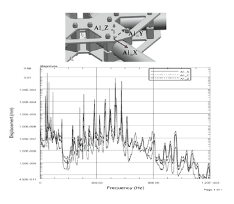
\includegraphics[width=4cm]{images/stage_system/design_graphs/vibrations_measurement.png}
%   \caption{ Measure of displacements [\textcolor{red}{CITE}].}
%   \label{fig:marginfig}
% \end{marginfigure}

%\end{itemize}

% \subsection{Synchronisation of Data Logging}
%     The data-logging activation file was coded in C++, and compiled into an executable via the MAVLink protocol. 
    
%     During operation, it simply toggles a pin (FMU Channel 6), which can then be detected by the data acquisition system in order to begin and end the logging. The executables are called: 
    
%     \begin{minted}
%     [
%     frame=lines,
%     framesep=2mm,
%     baselinestretch=1.2,
%     bgcolor=LightGray,
%     fontsize=\footnotesize,
%     linenos
%     ]
%     {python}
%     # RESET PIN (0) AT STARTUP, THEN POWER UP DAQ
%     nsh> px4_slice_disconnect
%     # SET PIN (1) TO START LOGGING 
%     nsh> px4_slice_disconnect
%     \end{minted}
    
    

% \begin{itemize}
%     \item Logging UORB Topics: Procedure
%     \item Logging Arduino Sensors: Procedure and Syncing Logs
%     \item Logging Slice Sensors: Procedure and Syncing Logs
%     \item Starting and Ending the Log
%     The Data Logging script is executed in the Mavlink Console.
%         \begin{minipage}{0.5\textwidth}
%           \centering
%           \begin{minted}{html}
%           nsh> px4_disconnect_slice 
%           \end{minted}
%           \captionof{listing}{Sub caption}
%          \end{minipage}
%          \begin{minipage}{0.5\textwidth}
%           \centering
%           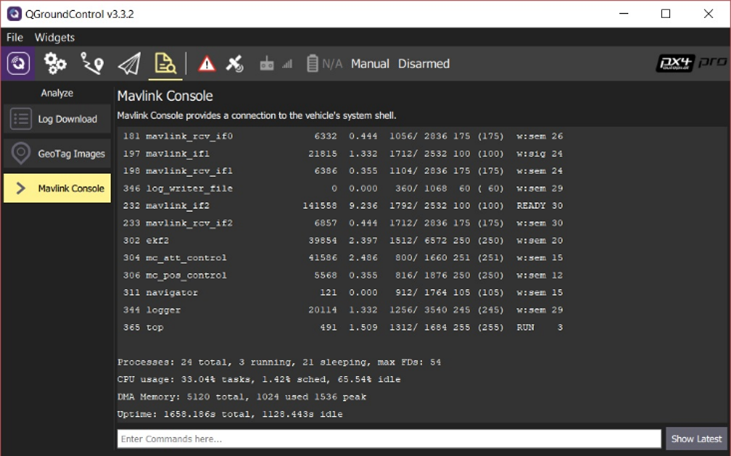
\includegraphics[width=4cm]{images/stage_graphs/environment_results/logging.png}
%           \captionof{listing}{Another sub caption}
%          \end{minipage}
%          \captionof{listing}{SomeCaption}
%           \label{lst:representation_examples}
          
%         \begin{figure*}[h]
%             \centering
%             \includegraphics[width=8cm]{images/stage_graphs/environment_results/logging.png}
%             \caption{Mavlink Console (QGC) where the Data Logging script is executed.}
%         \end{figure*}
% \end{itemize}



% \begin{figure*}[h]
%     \centering
%     \includegraphics[width=8cm]{images/fimi1.jpg}
%     \includegraphics[width=8cm]{images/fimi2.jpg}
%     \caption{Selected UAV, the FIMI X8 SE(a) with a Mini used as a Payload (b)}
% \end{figure*}

\pagebreak
\section{Semi-autonomous scan of a zone}\label{section:environment}

% \boolean{grayscale}{true}
% \newenvironment{mytikz}{%
%     \begin{tikzpicture}
%     \ifthenelse{\boolean{grayscale}}{\selectcolormodel{gray}}{images/stage_system/stage_ref/factories.jpg} 
%     }
%     {\end{tikzpicture}}
%\setboolean{grayscale}{true}% for the black & white version   
  %\selectcolormodel{gray}
  %\ifthenelse{\boolean{grayscale}}{\selectcolormodel{gray}}{} 
  
\begin{marginfigure}%
  \includegraphics[width=5cm]{images/stage_system/stage_ref/factories_bw.jpg}
  \caption{ Factories besides a body of water. Many organisations aim to use drones to scan air pollution in the surrounding areas.}
  \label{fig:factories}
\end{marginfigure}


%\subsection{Context}
% {field_scan_why}
Environmental sensing usually requires substantial time for data collection or more distributed sensing systems.  The use of atmospheric sensors is a major element in remote sensing \cite{metrology_survey}. With a platform that can carry multiple types of sensors, a simple field scan can help understand the limitations of a drone task, and the potential for further operations. As an air monitoring solution, this demonstration can be extended to industrial-type solutions, such as air pollution monitoring \cite{sørensen_jacobsen_hansen_2017}. All these factors show that drones form part of a trend towards service automation for industrial purposes. 

% {field_scan_overview}
We do remote sensing upon a UAV to simplify the task of environment sensing. A drone is equipped with remote sensors. It is flown in a field where it detects physical changes in the environment: lighting, humidity, and temperature.  This data is then processed to determine the effectiveness of the survey. A presentation video is available (Google Drive) \cite{fieldscan_video}. The experiment data is available on Google Drive \cite{fieldscan_dataset}.

\subsection{DAQ System Design}  

This section documents the design of the Atmosphere Data Payload selected in Section \ref{section:sensor_system}. It is composed of three stages.
            
\begin{figure*}[!h]
    \raggedright
    \hspace{1.7cm}
    {\includegraphics[width=8cm]{images/stage_system/drone_setup/payload_onboard.png}}
    
    \caption{Preparation of Atmospheric Data Collection.}
    \label{fig:prep_atmospheric}
\end{figure*}

The payload is installed on the drone in Step 1. Flight procedures are designed in Step 2. The DAQ Activation is done in Step 3.

\subsubsection{System for Low-Cost Sensors}\label{section:msp_daq}
        %%%%%%%%%%%%%%%%%%%%%%%%%%%%%%%%%%%%%%%%%%%%%%%%%%%%%%%%%%%%%%%%%%%%%%%%%%%%%%%%%%%%%%%%%
\begin{marginfigure}%
  \hspace{0.5cm}
  \includegraphics[width=3cm]{images/stage_system/nano_pic.jpg}
  \caption{ The Arduino Nano: a small, breadboard-friendly, rapid prototyping board \cite{arduino_docs}.}
\end{marginfigure}
            
        The Arduino sensor range is chosen for prototyping for its low-cost sensors. Using an Arduino Nano \cite{arduino_docs}, such sensors can be easily integrated. The Arduino Nano is sold as a small, complete, and breadboard-friendly board based on Arduino's larger counterpart, the ATmega328. It only weighs 7g with minimal volume.

  
% \subsubsection{System for High-Sensitivity and High Sampling Rate}     
%         %%%%%%%%%%%%%%%%%%%%%%%%%%%%%%%%%%%%%%%%%%%%%%%%%%%%%%%%%%%%%%%%%%%%%%%%%%%%%%%%%%%%%%%%%
%             \begin{marginfigure}%
%               \hspace{0.5cm}
%               \includegraphics[width=3cm]{images/stage_system/SLICE-MICRO.jpg}
%               \caption{ The DTS SLice Micro: a miniature, modular, rugged data acquisition system \cite{slice_docs}.}
%             \end{marginfigure}
%         The Micro Slice by DTS \cite{slice_docs} is a modular data acquisition system featuring unmatched flexibility and reliability for critical test applications. UAV flight is once such application that requires a small, reconfigurable and robust system. They offer a wide range of sampling rates of 10Hz to 500kHz and data storage of up to 16Gb. The Slice is used in aerospace analysis, automotive safety, biomechanics, and other safety-critical applications. 
        
%         % This is a product that is commercialised by Alliantech, and therefore an opportunity to explore an integration onboard a UAV. 

\subsubsection{Module Design}  

\begin{marginfigure}%[!h]
    \raggedright
    {\includegraphics[width=5.5cm]{images/stage_system/drone_setup/payload_onboard1.png}}
    \caption{Setup Step 1.}
    \label{fig:zone_scan_prep1}
\end{marginfigure}



Two separate modules are designed for the Atmospheric Data and the Vibration Data. In each, an independent battery powers the logging unit, and the sensors attached to it. The Pixhawk board is included in the first system since some the GPS and luminosity sensor are logged via the Pixhawk board.

\begin{figure*}[!h]
    \raggedright 
    \subfloat[Arduino DAQ Components]{\includegraphics[height=6cm]{images/stage_system/arduino_arch.PNG}}
    \subfloat[DAQ Integration on the UAV]{\includegraphics[height=6cm]{images/stage_graphs/environment_results/arduino_setup.jpg}}
    \caption{Arduino DAQ setup for field scan}
    \label{connections:arduino}
\end{figure*}
 

\pagebreak
\subsubsection{DAQ Control Layer}  

\begin{marginfigure}%[!h]
    \raggedright
    {\includegraphics[width=5.5cm]{images/stage_system/drone_setup/payload_onboard2.png}}
    \caption{Setup Step 2.}
    \label{fig:zone_scan_prep2}
\end{marginfigure}


The DAQ is configured to activate and deactivate the datalogging process on command. To achieve this, we use custom activation firmware on the PX4 operating system.  

% \begin{marginfigure}%[h]
%     \raggedright
%     \includegraphics[width=4cm]{images/stage_system/switch-setup.jpg}
%     \includegraphics[width=4cm]{images/stage_system/switch_view.jpg}
%     \caption{Switch Configuration Screen.}
%     \label{fig:RC_screen}
% \end{marginfigure}
  

\begin{table*}[!h]
  %\raggedright
  \footnotesize%
  \begin{flushleft}
    \begin{tabular}{lccccl}
      \toprule
      Boards                     & Switch  & Activation & Deactivation & Prior to Activation \\
                                    % & Acceleration & Sensors & Sensor & System\\
      \midrule
    %   1. SLICE Micro    & 2-3    &  Custom App  & Custom App    & Arming  \\
      2. Arduino Nano   & 2-2    &  On boot         & On shutdown    & None  \\
      3. Pixhawk        & 2-1    &  On boot         & On shutdown       & None \\
    %   Requires a Modular Setup      & \CIRCLE    &  \Circle & \CIRCLE & \CIRCLE\\
    %   \toprule
    %   Selection                     &  \ding{51} &  \ding{55} &  \ding{51} &  \ding{51} \\
      \bottomrule
    \end{tabular}
  \end{flushleft}
  \caption{DAQ Activation Procedure.}
  \label{tab:daq_activation}
\end{table*}

The data-logging activation file was coded in C++, and compiled into an executable via the MAVLink protocol. During operation, it toggles a pin (Pixhawk's FMU Channel 6), which is then detected by the Arduino Nano in order to begin and end the logging on the Datalogger. 

A separate custom logger detects Arduino activation and records its timestamp in the PX4 debug log.

\pagebreak
\subsection{Sensor System Evaluation}
\subsubsection{Aim}
Using three separate atmospheric variables, we determine the accuracy of the drone sensing solution.

\subsubsection{Prediction}

Sunlit and shaded regions were scanned for relative humidity, luminosity and ambient temperature. The drone’s flightpath is changed randomly by the operator to create region overlaps. The trajectory plots demonstrate any inconsistencies in the readings. We determine the maximal variation per second and per meter as a measure of the fluctuations in lighting and in temperature.

\subsubsection{Method}

% \subsubsection{UAV System Configuration}

%\subsubsection{Onboard Sensor Integration}
\begin{marginfigure}%[!h]
    \raggedright
    {\includegraphics[width=5.5cm]{images/stage_system/drone_setup/payload_onboard3.png}}
    \caption{Setup Step 3.}
    \label{fig:zone_scan_prep3}
\end{marginfigure}


\textit{Measurement Equipment Setup} \hspace{0.3cm} Instruments that were used in the system are pictured in Figure \ref{connections:arduino}. These include the DH11 Temperature and Humidity sensor, as well as a 5mm LDR Luminosity Sensor, and finally, the companion GPS. A particularity is that the DH11 is attached to the Arduino Board, and Logged with the use of an Arduino Data Logger, while the 5mm LDR is connected to an ADC input on the Pixhawk board, containing a self-enclosed data logger.

% \begin{figure*}[h]
%     \raggedright
%     %\hspace*{\fill}   % maximize separation between the subfigures
%     \subfloat[FFT Graph for  Payload A and Reference]{\includegraphics[height=4cm]{images/stage_system/design_graphs/fourier_transform.png}}
%     \subfloat[FFT Graph for Payload B and Reference]{\includegraphics[height=4cm]{images/stage_system/design_graphs/fourier_transform.png}}
%     \\
%     \subfloat[FFT Graph for Payload B and Reference]{\includegraphics[height=4cm]{images/stage_system/design_graphs/fourier_transform.png}}
%     \subfloat[Gain difference between the two payloads]{\includegraphics[height=4cm]{images/stage_system/design_graphs/freqresponse_payload.png}}
%     \caption{Development of the Gain Graphs to compare Payload A and B}
% \end{figure*}

The Pixhawk logger supports 100Hz data logging while the Arduino data logger averages at 10Hz logging. Both data loggers support Micro SD cards with a capacity of up to 64GB to store high-resolution video data, photos and flight telemetry.


\textit{Experiment Procedure} \hspace {0.3cm} The flight takes place in an empty field of approximately 100x60m, identified for the differences in lighting between the tree shade and the sunlit field. The drone is piloted by hand. This requires a certain method:

\begin{enumerate}
    \item System checks (battery monitor, screws, etc.)
    \item Activating the drone.
    \item Drone takeoff and moving to an altitude of 2m.
    \item Altitude lock.
    \item Activating the Arduino data acquisition with a PX4 trigger application.
    \item Piloted flight across the field, along sunlit and shaded regions.
\end{enumerate}

% \subsubsection{Automation procedures}

% To automate the logging process, several executables are developed:

% \begin{itemize}
%     \item Activation of the Pixhawk data logger upon system startup, a functionality designed by QGroundControl.
%     \item Activation of the Arduino data logger via a trigger executable, available in Appendix A, Section \ref{logger:arduino}.
%     \item Custom Pixhawk messages to timestamp the activation time of the Arduino, available in Appendix A, Section \ref{logger:pixhawk}.
% \end{itemize}



\begin{marginfigure}%[!h]
    \raggedright
    %\includegraphics[width=3cm]{images/px41.jpg}
    \includegraphics[width=5cm]{images/stage_graphs/environment_results/Flight_Drone.png}
    %\includegraphics[width=9cm]{images/stage_graphs/vibration_results/footsteps.png}
    \caption{Presentation video \cite{fieldscan_video} }
\end{marginfigure}

\textit{Data collection} \hspace{0.3cm} The data was collected on 24 August 2021, over an empty field of approximately 100x60m. Both the lighting and the GPS data are taken from the Pixhawk Log. They were both sampled at a frequency of 98 Hz. The Arduino Logger was activated  248s after the Pixhawk Logger. The Arduino Logger was active for a duration of 712 seconds, of which 464s are common to both boards. Both the temperature and the humidity are taken from the Arduino Datalogger. They were both sampled at a frequency of 11.7 Hz.\\

\textit{Dataset} \hspace{0.3cm}  A presentation video is available (Google Drive) \cite{fieldscan_video}. The experiment data is available on Google Drive \cite{fieldscan_dataset}.

%The Pixhawk board was on for a duration of 780 seconds.


%\subsubsection{Flight Location}

        % \begin{figure*}[h]
        %     \raggedright
        %     \includegraphics[width=10cm]{images/stage_graphs/environment_results/test_site.png}
        %     \caption{Flight site.}
        % \end{figure*}

    % ADD IF HAVE TIME TO DO THIS.     % URGENT !!!!
% \subsubsection{Sensor Selection}
%     \begin{itemize}
%         \item DH11.
        
%         \item LDR 5mm.
%     \end{itemize}
    % ADD IF HAVE TIME TO DO THIS.
    %\item QGroundControl for Designing new Trajectories
    
    % ADD IF HAVE TIME TO DO THIS.
    %\item Piloting from Operator: Flight Modes

    % ADD IF HAVE TIME TO DO THIS.
    %\item Safety Settings
        % \begin{figure*}[h]
        %     \centering
        %     \includegraphics[width=8cm]{images/stage_graphs/environment_results/safety.png}
        %     \caption{Safety Settings Page (QGC) where the Geofence and Return to Home are configured.}
        % \end{figure*}
    
    % Transition this to System Overview    
    %\item Payload Setup
        % \begin{figure*}[h]
        %     \centering
        %     \includegraphics[width=8cm]{images/stage_graphs/environment_results/Arduino_setup.png}
        %     \caption{Elements of the Arduino Payload Setup.}
        % \end{figure*}
    
%\end{itemize}
\pagebreak
\subsubsection{Results}

% \begin{marginfigure}%
%   \includegraphics[width=4cm]{images/stage_graphs/environment_results/Flight_Drone.png}
%   \caption{ Full flight compilation \href{https://drive.google.com/file/d/1rM8Lbhx0dXqLEne-o6SuOQslv0_WiJV_/view?usp=sharing}{available here}.}
%   \label{video:scanning}
% \end{marginfigure}

\textbf{Timeline of Environment Sensor Readings} \hspace{0.3cm} There is a stark contrast between sunny and shady regions in the data.

% The timestamps of the Arduino and Pixhawk loggers were correlated with the help of the debugger messages on the control layer.

%% This script is documented here \appendixcode{\ref{logger:pixhawk}}.

\begin{figure*}[!h]
    \raggedright
    \includegraphics[width=12cm]{images/stage_graphs/environment_results/arduino_plot.png}
    \caption{Temperature, Humidity and Lighting Recordings during Flight}
\end{figure*}


 This is a change of 20\% of the luminosity range, where sunny regions saturate the sensor, and shady regions are marked by sudden drops. 


\textbf{Trajectory Plot} \hspace{0.3cm} Figure \ref{fig:lighting_field} plots the lighting readings over the trajectory.
% The exact code is replicable and documented here (\textcolor{teal}{Appendix A, Section \ref{code:map}}).

% To obtain the following trajectory plots, drone positions are rotated by 45 degrees, corresponding to the orientation of the background picture in a grid reference system.  

\begin{figure*}[!h]
    \raggedright
    \begin{minipage}{1.0\textwidth}
    \centering
    \subfloat[Trajectory with Lighting as a Colour]{\includegraphics[width=9cm]{images/stage_graphs/environment_results/Lighting_field_plot.png}}\\
    \subfloat[Trajectory with Temperature as a Colour]{\includegraphics[height=3.3cm]{images/stage_graphs/environment_results/Temperature_field_plot.png}}\\
    \subfloat[Trajectory with Humidity as a Colour]{\includegraphics[height=3cm]{images/stage_graphs/environment_results/Humidity_field_plot.png}}
    \end{minipage}
    \caption{Plot of Drone GPS Position during Flight with Lighting represented as a Colour}
    
    \label{fig:lighting_field}
\end{figure*}

% The temperature and humidity plots are plotted in space as a rough measure of their accuracy.
% https://www.mouser.com/datasheet/2/758/DHT11-Technical-Data-Sheet-Translated-Version-1143054.pdf
        % https://www.canva.com/design/DAEr-xg390A/479cjxgtYK5CUtGn_sDufg/edit
% time per 100: 11.251628637313843 in minutes: 32.85850616383553
% 122.63130235463619 is max light change/m
% 2.901681308865982 is min light change/m.
% 9.618320610687025 is max light change/s.
% 0.2290076335877841 is min light change/s.
% LUX RANGE is 1.440722556835771 to 272.2153652634392
% \begin{figure*}[!h]
%     \raggedright
%     \begin{minipage}{1.0\textwidth}
%     \centering
%     \hspace{2cm}\subfloat[Trajectory with Temperature as a Colour]{\hspace{-2cm}\includegraphics[height=4.3cm]{images/stage_graphs/environment_results/Temperature_field_plot.png}}\\
%     \hspace{2cm}\subfloat[Trajectory with Humidity as a Colour]{\hspace{-2cm}\includegraphics[height=4cm]{images/stage_graphs/environment_results/Humidity_field_plot.png}}
%     \end{minipage}
%     \caption{Plot of Drone GPS Positions during Flight}
%     \label{fig:lighting_field}
% \end{figure*}

This confirms that the data is very sensitive to lighting differences. The darker patches in the sunlit area might be explained by the passage of clouds during the procedure. 

\textbf{\Copy{sensor_rate_second}{Sensor Range in Time}} A first graph presents the magnitude of the changes in light and temperature, by computing their rates of change over time. The magnitudes are normalized by their operating ranges: 20-90\% of Relative Humidity for the DHT11 sensor, 20-150mV of ADC voltage for the LDR sensor.

\begin{equation}
{\frac{\Delta{r}}{{t}}} = 
{\frac{r_{f} - r_{i}}{r_{max}-r_{min}} * 100}
\end{equation}

\begin{figure*}[!h]
    \raggedright
    \hspace{0.5cm}\subfloat[Fluctuations per Second]{\hspace{-0.5cm}\includegraphics[height=3.2cm]{images/stage_graphs/environment_results/sensor_speeds.png}}
    \hspace{0.5cm}\subfloat[Fluctuations per Meter]{\hspace{-0.5cm}\includegraphics[height=3.2cm]{images/stage_graphs/environment_results/changes_m2.png}}
    % \includegraphics[width=11cm]{images/stage_graphs/environment_results/sensor_speeds.png}
    \caption{Fluctuations in Measurements of LDR and DHT11 Sensors}
    \label{fig:reading_variations}
\end{figure*}

According to (a), the maximum values suggest that the LDR sensor records changes of \Copy{LDR_rate_second}{0.23 \% to 0.69 \% shift in operating range/reading} vs the DHT11 sensor's \Copy{DHT11_rate_second}{0.14\% to 6.62 \% shift in operating range/reading}. The temperature and humidity vary less rapidly, and this is very apparent in the plots. 

% 45.555902156511415 is max temp change/m.
% 0.06268337269712651 is min temp change/m.
% 6.619718309859154 is max temp change/s.
% 0.14084507042253222 is min temp change/s.





% LUX RANGE is 57.914912336320675 to 270.27642001285227
% 2.916 to 8.7646 mV per meter, given that the voltage range is 130mV.
% 0.229 \% to 0.687 \% of the LDR operating range per increment.

% 8.764699300267512 is max light change/m.
% 2.9165350248404134 is min light change/m.
% 0.6870229007633577 is max light change/s.
% 0.2290076335877841 is min light change/s.

\textbf{\Copy{sensor_rate_meter}{Sensor Range in Space}} To better evaluate the sensing speed, we investigate the maximum fluctuations per second, and then per meter. This data recording speed is used in (b) in coordination with the drone velocity as recorded by the Pixhawk setup, in order to obtain fluctuations per meter, independent from speed. This is done with the following equations.

\begin{equation}
{\frac{\Delta{r}}{{m}}} = 
{\frac{r_{f} - r_{i}}{t_{f} - t_{i}}}* {\frac{1}{\bar{v}}}
\end{equation}

\begin{marginfigure}%[!h]
    \raggedright
    %\includegraphics[width=3cm]{images/px41.jpg}
    \includegraphics[width=5cm]{images/stage_graphs/environment_results/lux_voltage.png}
    %\includegraphics[width=9cm]{images/stage_graphs/vibration_results/footsteps.png}
    \caption{Empirical relationship \cite{ldr_testing} }
\end{marginfigure}

The following equation is taken from \cite{ldr_testing}, whereas \citename{ldr_testing}{author} determines an empirical formula to convert the ADC voltage to lux for the Arduino's Light Dependent Resistor module:
\begin{equation}
    \log{(L_{lux})} = -1.4*\log\{ \max{ |{V_{adc}}| } \}+7.098
\end{equation}

Whereas the LDR sensor records \Copy{LDR_rate_meter}{57.915-270.276 lux variation/meter}, the DHT11 detects \Copy{DHT11_rate_meter}{0.062-45.556 \% of Relative Humidity variation/meter}. This shows the range of local changes over the field and it seems reasonable for stark changes in light vs more gradual changes in humidity.

% \begin{figure*}[!h]
%     \raggedright
%     \includegraphics[width=11cm]{images/stage_graphs/environment_results/changes_m2.png}
%     \caption{Fluctuations in Measurements of LDR and DHT11 Sensors per Meter}
%     \label{fig:lighting_field}
% \end{figure*}




\pagebreak



% % TO ADD BACK
% \begin{figure*}[!h]
%     \raggedright
%     %\includegraphics[width=4cm]{images/stage_graphs/environment_results/lighting_field_1.png}
%     \subfloat[]{\includegraphics[width=6cm]{images/stage_graphs/environment_results/Temperature_field_plot.png}}
%     \subfloat[]{\includegraphics[width=6cm]{images/stage_graphs/environment_results/lighting_field_3_zoom.png}}
%     \caption{Progressive close-ups of field}
% \end{figure*}

% \begin{figure*}
%   \raggedright
%   \begin{subfigure}{0.7\linewidth}
%     \centering
%     \includegraphics[width=\linewidth]{images/stage_graphs/environment_results/lighting_field_2.png}
%     \caption{}
%     \label{Fig2a}
%   \end{subfigure}\par
%   \medskip
%   \begin{subfigure}{0.7\linewidth}
%     \centering
%     \includegraphics[width=\linewidth]{images/stage_graphs/environment_results/lighting_field_2.png}
%     \caption{}
%     \label{Fig2b}
%   \end{subfigure*}
%   \caption{Pictures of animals}
%   \label{fig:animals}
  



\subsection{Discussion}

The proposed UAV architecture has proven itself effective at capturing fluctuating environment data. When examining the luminosity readings, the measurements are very consistent with shade/light regions, by changes of as much as 20\% of the luminosity range. Sunny regions saturate the sensor, and shady regions are marked by sudden drops. This suggests a high accuracy, especially seen as the drone was piloted by hand. 

% {field_scan_evaluation_conclusion}
The luminosity plot demonstrates very precise readings despite the drone's velocity. This is facilitated by rapid data logging at 100Hz. The fact that the drone was piloted by hand, on an arbitrary path with region overlaps, illustrates plainly how mobile mapping is a worthwhile tool for rapid data collection.

There is much less of a correlation between the readings and their position in space. We suggest two potential issues with the DH11 sensor:
\begin{itemize}
    \item Movement may affect the temperature and humidity. We recommend to further investigate how the readings vary with altitude, speed and acceleration.
    \item Heat convection on the drone and the sensor itself may be recorded by the sensor instead of environment temperature. We recommend to further investigate how accumulated heat affect the readings.
\end{itemize}

Additionally, this experiment demonstrates that a payload drone can be extended to other types of sensors for other applications. The data acquisition setup proves to be functional. This setup was developed prior to the experiment with the goal to integrate many other types of sensors. 

The flight was quite smooth and simple to undertake. As opposed to conventional means of environmental sensing \cite{xiang_xia_zhang_2020}, this flight requires no site preparation. This is largely due to the selected drone system, as well as the work done to automate the data acquisition procedures.

% {field_scan_approach}
This procedure was greatly assisted by the datalogger, whereas GPS data and atmospheric data could be correlated without major issues. The correlation between different elements have uncovered a topography in an unexpectedly accurate manner. As we examine the systems that aid in practice, we note the importance of the drone as a platform for capturing scans of a 3 dimensional environment in a rapid, and timely manner. At the time of writing, Alliantech is compiling a marketing video for this environment sensing solution.


%   %   %   %   %
\pagebreak
\section{Structural Inspection of Vibrations}\label{section:vibrations}

\begin{marginfigure}%[h]
    \raggedright. 
    \includegraphics[width=5cm]{images/stage_system/water-outlet_bw.jpg}
    \caption{Instance of a water outlet where a drone can land and monitor water flow.}
    \label{fig:outletpipe}
\end{marginfigure}    

We sometimes wish to monitor the vibrations of a large structure. With conventional methods, this usually requires reaching the zone by foot and attaching the sensor in some form, and these pipes may be in dangerous or inconveniently placed. For example, it is a challenging task to monitor water flow through a sewer outlet pipe (Figure \ref{fig:outletpipe}). In this project, we explore sensor placement with a UAV to demonstrate a simpler way to do vibration monitoring. 

We designed a drone to land on the measurement site. To do this, a drone is equipped with the vibration data acquisition systema. A vibration probe mount is designed to fit the accelerometer on a leg of the drone. This full system is evaluated, first to determine whether it detects footsteps accurately, and the second to determine a range of frequencies at which the setup remains functional. 




\subsection{DAQ System Design}

This section documents the design of the Vibration Data Payload selected in Section \ref{section:sensor_system}. It is composed of three stages.
            
\begin{figure*}[!h]
    \raggedright
    \hspace{1.7cm}
    {\includegraphics[width=8cm]{images/stage_system/drone_setup/prep_diagram2.png}}
    
    \caption{Preparations for Vibration Data Collection.}
    \label{fig:prep_diagram}
\end{figure*}

The payload is installed on the drone in Step 1. Flight procedures are designed in Step 2. The DAQ Activation is done in Step 3.

            \begin{marginfigure}%
              \hspace{0.5cm}
              \includegraphics[width=3cm]{images/stage_system/SLICE-MICRO.jpg}
              \caption{ The DTS SLice Micro: a miniature, modular, rugged data acquisition system \cite{slice_docs}.}
            \end{marginfigure}
  

\subsubsection{System for High-Sensitivity and High Sampling Rate}     
%%%%%%%%%%%%%%%%%%%%%%%%%%%%%%%%%%%%%%%%%%%%%%%%%%%%%%%%%%%%%%%%%%%%%%%%

The Micro Slice by DTS \cite{slice_docs} is a modular data acquisition system featuring unmatched flexibility and reliability for critical test applications. UAV flight is once such application that requires a small, reconfigurable and robust system. They offer a wide range of sampling rates of 10Hz to 500kHz and data storage of up to 16Gb. The Slice is used in aerospace analysis, automotive safety, biomechanics, and other safety-critical applications. 
        
\subsubsection{Module Design}  

\begin{marginfigure}%[!h]
    \raggedright
    \hspace{1.5cm}
    {\includegraphics[width=5.5cm]{images/stage_system/drone_setup/payload_onboard1.png}}
    \hspace{1cm}\caption{Setup Step 1.}
    \label{fig:zone_scan_prep1b}
\end{marginfigure}


An independent module is designed for the Vibration Data. An independent battery powers the logging unit, and the sensors attached to it. The Pixhawk board is included in this system since the Slice is armed via the Pixhawk board.

\begin{figure*}[!h]
    \raggedright
    \includegraphics[height=5.3cm]{images/stage_system/slice_arch.PNG}
    \includegraphics[height=5.3cm]{images/stage_system/footstep_test.png}
    \caption{DTS Slice DAQ Subsystem}
    \label{connections:slice}
\end{figure*}
        
Instruments that were used in the system are pictured in Figure \ref{connections:slice}. These include a 3055B2T accelerometer and a data logging system. This accelerometer is directly connected to the DTS slice data acquisition system, which is a self-enclosed data logger.



\subsubsection{Drone Mount Design}


Hand probes are conventionally used to in frequency response tests on the terrain, as shown in Figure \ref{fig:handprobe}. This is used in our design to make contact between the drone and the ground. A mounting part is required to fix this hand probe to the drone. A part is designed and 3D printed for this purpose.

\begin{marginfigure}%[h]
    \raggedright
    \includegraphics[width=4cm]{images/stage_graphs/vibration_results/vibration_probe_use.jpg}
    \caption{A conventional vibration probe tip is pressed against a surface by hand.}
    \label{fig:handprobe}
\end{marginfigure}  

\begin{figure*}[!h]
    \raggedright
    \includegraphics[height=1.8cm]{images/stage_system/renders/accelerometer_mount/abs_side1.JPG}
    \includegraphics[height=1.8cm]{images/stage_system/renders/accelerometer_mount/abs_side2.JPG}
    \includegraphics[height=1.8cm]{images/stage_system/renders/accelerometer_mount/profile.JPG}
    \includegraphics[height=1.8cm]{images/stage_system/renders/accelerometer_mount/steel_corner.JPG}
    \caption{Renders of vibration probe mount.}
\end{figure*}

This mount places itself in the place of a drone leg (Figure \ref{connections:slice}). It measures the same size as the other legs, such that the drone's weight is equally distributed on the drone legs.

\begin{figure*}[!h]
    \raggedright
    \hspace{2cm}
    \includegraphics[width=6cm]{images/stage_graphs/vibration_results/vibration_test_drone.png}
    \hspace{2cm} \caption{Installation of External Accelerometer}
\end{figure*}

\subsubsection{DAQ Control Layer}  

\begin{marginfigure}%[!h]
    \raggedright
    {\includegraphics[width=5cm]{images/stage_system/drone_setup/payload_onboard2.png}}
    \caption{Setup Step 2.}
    \label{fig:vibration_prep3}
\end{marginfigure}


The DAQ is configured to activate and deactivate the datalogging process on command. To achieve this, we use custom activation firmware on the PX4 operating system.  

\begin{table*}[!h]
  %\raggedright
  \footnotesize%
  \begin{flushleft}
    \begin{tabular}{lccccl}
      \toprule
      Boards                     & Switch  & Activation & Deactivation & Prior to Activation \\
                                    % & Acceleration & Sensors & Sensor & System\\
      \midrule
      1. SLICE Micro    & 1-1    &  Custom App  & Custom App    & Arming  \\
    %   2. Arduino Nano   & 1-2    &  On boot         & On shutdown    & None  \\
      2. Pixhawk        & 1-3    &  On boot         & On shutdown       & None \\
    %   Requires a Modular Setup      & \CIRCLE    &  \Circle & \CIRCLE & \CIRCLE\\
    %   \toprule
    %   Selection                     &  \ding{51} &  \ding{55} &  \ding{51} &  \ding{51} \\
      \bottomrule
    \end{tabular}
  \end{flushleft}
  \caption{Flight Mode Assignment for RC Controller.}
  \label{tab:rc_assignment}
\end{table*}

The data-logging activation file was coded in C++, and compiled into an executable via the MAVLink protocol. During operation, it toggles a pin (the Pixhawk's FMU Channel 6), which is then detected by the data acquisition system in order to begin and end the logging. 

The Pixhawk logger is used to log debugging messages at 100Hz, while the Slice data logger ranges from  at 1kHz to 500kHz logging. The Pixhawk data logger is fitted with a 16Gb Micro SD card while the DTS slice supports up to 16Gb of memory.


\subsection{Experiment 1: Detection of Footsteps}

\begin{marginfigure}%[!h]
    \raggedright
    {\includegraphics[width=5cm]{images/stage_system/drone_setup/payload_onboard3.png}}
    \caption{Setup Step 3.}
    \label{fig:vibration_prep3}
\end{marginfigure}


\subsubsection{Experiment Procedure}
\textit{Flight Procedure}\hspace{0.3cm} The experiment is conducted indoors. 
As the subject of the experiment is the measurement of vibrations, a sequence of steps is put in place.

\begin{enumerate}
    \item The data acquisition system is activated.
    \item The drone is flown and lands. 
    \item The passer-by walks at 1m from the drone.
\end{enumerate}

\textit{Data Collection}\hspace{0.3cm} The DTS Slice is set up according to a few parameters. DAQ parameters are listed in Table \ref{tab:footstep_testsettings}. 

\begin{table*}[h]
  %\raggedright
  \footnotesize%
  \begin{flushleft}

    \begin{tabular}{ll}
      \toprule
      Test Description & Ground Accelerometer (ref)  \\
      \midrule
      Test Date                     &  23/08/2021 \\
      Test Time                     &  16:08:18 \\
    %   Test ID &   Flight3MOUSSE\_coupe  \\
      Sample Rate                   &  10000 Hz  \\
      Hardware AA Filter (-3dB)     & 2900    \\
      Data Channel Number           &	1    \\
      Channel Description           & 3055B2T\_REF   \\
        Software Filter (SAE Class)	&NONE \\
        Software Filter (-3dB)	&NONE \\
        Engineering Unit	&g \\
      Number of Pre-Zero Data Pts	& 0	  \\
      Number of Post-Zero Data Pts	& 240042	  \\
      Data Zero (CNTS)	            & 57 \\
    Scale Factor (EU/CNT)	        & 0.003781480491161	  \\
    Scale Factor (mV/CNT)	        & 0.378148049116135  \\
      \bottomrule
    \end{tabular}
  \end{flushleft}

  \caption{Parameters of the Footstep Detection Test.}
  \label{tab:footstep_testsettings}
\end{table*}
 
The DAQ was sampled at 10kHz. The anti-aliasing filter (AA), output scale factor and sampling rate are defined, among other factors.


\textit{Dataset} \hspace{0.3cm} The procedure was carried out on 23 August 2021 in an indoor parking space. The Google Drive experiment dataset \cite{vibrationmount_dataset} and a Youtube presentation video \cite{vibrationmount_video} are publicly available.

\subsubsection{Results}

The raw data is represented as the red markers in Figure \ref{fig:raw_footsteps}. 
% \begin{marginfigure}%[!h]
%     \raggedright
%     \includegraphics[width=3cm]{images/px41.jpg}
%     %\includegraphics[width=9cm]{images/stage_graphs/vibration_results/footsteps.png}
%     \caption{The procedure was carried out on 23 August 2021 in an indoor parking space. The Google Drive experiment dataset \cite{vibrationmount_dataset} and a Youtube presentation video \cite{vibrationmount_video} are publicly available.}
% \end{marginfigure}


% \begin{marginfigure}%[!h]
%     \raggedright
%     \includegraphics[width=5cm]{images/stage_graphs/vibration_results/vibration_test.png}
%     \caption{Vibrating Pot Experimental Setup}
% \end{marginfigure}

    
\begin{figure*}[!h]
    \raggedright
    \includegraphics[width=10cm]{images/stage_graphs/vibration_results/raw_footsteps.png}
    \caption{Raw data and final sensitivity curve}
    \label{fig:raw_footsteps}
\end{figure*}


% sos is [[ 7.78600798e-13  1.55720160e-12  7.78600798e-13  1.00000000e+00
%   -1.88142503e+00  8.85073379e-01]
%  [ 1.00000000e+00  2.00000000e+00  1.00000000e+00  1.00000000e+00
%   -1.89800683e+00  9.01707920e-01]
%  [ 1.00000000e+00  2.00000000e+00  1.00000000e+00  1.00000000e+00
%   -1.92944092e+00  9.33232523e-01]
%  [ 1.00000000e+00  2.00000000e+00  1.00000000e+00  1.00000000e+00
%   -1.97213843e+00  9.76034773e-01]
%  [ 1.00000000e+00 -2.00000000e+00  1.00000000e+00  1.00000000e+00
%   -1.99937808e+00  9.99378183e-01]
%  [ 1.00000000e+00 -2.00000000e+00  1.00000000e+00  1.00000000e+00
%   -1.99947564e+00  9.99475739e-01]
%  [ 1.00000000e+00 -2.00000000e+00  1.00000000e+00  1.00000000e+00
%   -1.99965225e+00  9.99652352e-01]
%  [ 1.00000000e+00 -2.00000000e+00  1.00000000e+00  1.00000000e+00
%   -1.99987846e+00  9.99878558e-01]] done
  
This raw data has considerable drift, which is due to an uncalibrated tool. This is a common issue when measuring with a single accelerometer as per \cite{gait_analysis}. To mitigate this drift, we make use of a Butterworth band-stop filter in Python, as it has a maximally flat frequency (ie. no ripples in the passband). This makes it one of the most popular and used band-stop filters.

\begin{figure*}[!h]
\raggedright
    \begin{minipage}{1.0\textwidth}
    \begin{minted}
    [
    frame=lines,
    framesep=2mm,
    baselinestretch=1.2,
    %bgcolor=LightGray,
    fontsize=\footnotesize,
    linenos
    ]
    {python}
    
    filtered_data = butter_bandpass_filter(raw_data, start_hz=7, 
                    end_hz=12, sample_hz=25000, order=5)*0.8
    \end{minted}
    %\caption{Example of Action Concurrence Code.}
    % \captionof{minted}{\textbf{Template 3:} Band-pass Butterworth Filter.}

    \caption{Parameters for Band-stop Butterworth Filter}
    \end{minipage}
\end{figure*}    
% \begin{equation}
% temp = butter_bandpass_filter(slice_array, 7, 12, 10000, order=5)*0.8
% \end{equation}

The filter is run between 7Hz and 12Hz, on a sampling frequency of 25kHz. The filter's transfer function is:

\begin{equation}
% G(\omega) = \frac{1}{\sqrt{1+\omega^{2n}}} \text{ with } n=7 \text{ and } \omega_{1} = 2\pi(7), \omega_{2} = 2\pi(12)
% H(z) = (\frac{1 }{z^{-2}-1.881z^{-1}+0.885})
% % (\frac{z^{-2}+2z^{-1}+1}{z^{-2}-1.898z^{-1}+0.9017})(\frac{z^{-2}+2z^{-1}+1}{z^{-2}-1.929z^{-1}+0.9332})
% (\frac{z^{-2}+2z^{-1}+1}{z^{-2}-1.972z^{-1}+0.976})^3(\frac{z^{-2}-2z^{-1}+1}{z^{-2}-1.999z^{-1}+0.993})^4 \text{ with } n=7 \text{ and } \omega_{1} = 2\pi(7), \omega_{2} = 2\pi(12)
H(z) = %(\frac{1 }{z^{-2}-1.881z^{-1}+0.885})
% (\frac{z^{-2}+2z^{-1}+1}{z^{-2}-1.898z^{-1}+0.9017})(\frac{z^{-2}+2z^{-1}+1}{z^{-2}-1.929z^{-1}+0.9332})
\frac{(z^{-2}+2z^{-1}+1)^3}{(z^{-2}-1.9z^{-1}+0.9)^4}
% (\frac{z^{-2}-2z^{-1}+1}{z^{-2}-2z^{-1}+1})^4 
% \text{ with } n=7 \text{ and } \omega_{1} = 2\pi(7), \omega_{2} = 2\pi(12)
\end{equation}

    % \begin{minted}
    % [
    % frame=lines,
    % framesep=2mm,
    % baselinestretch=1.2,
    % bgcolor=LightGray,
    % fontsize=\footnotesize,
    % linenos
    % ]
    % {python}
    
    % from scipy.signal import butter, sosfilt, sosfreqz
    
    % def butter_bandpass(lowcut, highcut, fs, order=5):
    %         nyq = 0.5 * fs
    %         low = lowcut / nyq
    %         high = highcut / nyq
    %         sos = butter(order, [low, high], analog=False, btype='bandstop', output='sos')
    %         return sos
    
    % def butter_bandpass_filter(data, lowcut, highcut, fs, order=5):
    %         sos = butter_bandpass(lowcut, highcut, fs, order=order)
    %         y = sosfilt(sos, data)
    %         return y
    
    % temp = butter_bandpass_filter(slice_array, 7, 12, 10000, order=5)*0.8
    % \end{minted}
    % %\caption{Example of Action Concurrence Code.}
    % \captionof{minted}{\textbf{Template 3:} Band-pass Butterworth Filter.}
    
The result is the following graph. 

\begin{figure*}[!h]
    \raggedright
    \includegraphics[width=10cm]{images/stage_graphs/vibration_results/filtered_footsteps.png}
    \caption{Filtered vibration curve}
    \label{fig:filtered_footsteps}
\end{figure*}

A single footstep is isolated from 23s to 28s. This data shows each footstep clearly with a gradual increase in signal amplitude (energy) followed by a gradual decrease. This same behaviour is seen in other parts of the rectified data. 



%(\textcolor{teal}{Appendix A, Section \ref{code:bandpass}})
\begin{figure*}[!h]
    \raggedright
    \includegraphics[width=10cm]{images/stage_graphs/vibration_results/footsteps_sequence.png}
    \caption{Inspection of a set of footsteps}
\end{figure*}

\begin{marginfigure}%[h]
    \raggedright \vspace{1cm}
    \includegraphics[width=6cm]{images/stage_graphs/vibration_results/reference_footsteps_bw.png}
    \caption{Footsteps as detected by \cite{gait_analysis}}
    \label{fig:footstep_reference1}
\end{marginfigure}  

The raw floor vibration signal behaves similarly to those in Figure \ref{fig:footstep_reference1} with footsteps increasingly far from the sensor. The decrease in signal amplitude (energy) correlates with increasing footstep-sensor distance.

\subsubsection{Hypothesis Validation}
The final graph shows footsteps quite neatly as they approach and leave the accelerometer. The hypothesis is therefore valid, and further discussion features in the Chapter Discussion, Section \ref{section:discuss_vibrations}.


% % EVAL
% This data was processed to remove any data ...

% \begin{figure*}[h]
%     \centering
%     \includegraphics[width=9cm]{images/stage_graphs/vibration_results/footsteps.png}
%     \caption{Footstep Data fitted with a BandPass Filter between 0.5 and 30Hz.}
% \end{figure*}

\subsection{Experiment 2: Sensor Sensitivity Evaluation}

Vibration tests reproduce the vibrations undergone by goods during transport. It is a good design practice to ensure the resonant frequencies are well above any vibration loads the product is likely to experience.

In order to perform these tests, there are different types of machines, such as the vertical vibration testing systems that only have one degree of freedom, or vertical, pitch and roll systems which have three degrees of freedom and very accurately reproduce the vibrations suffered during the transportation of goods \cite{safe_load_testing_technologies_2021}. 

\subsubsection{Procedure}
\textit{Experiment Equipment}\hspace{0.3cm} A vibration shaker is a device used in vibration testing to excite a structure. The shaker can perform a sinusoidal sweep, that is, a sinusoid whose frequency varies with time. This will reveal a resonant frequency, which means the vibration induced displacements are maximized. 

\begin{figure*}[!h]
    \raggedright
    % \includegraphics[width=8cm]{images/stage_graphs/vibration_results/vibration_test.png}
    \includegraphics[width=11cm]{images/stage_graphs/vibration_results/vibration_test_drone.png}
    \caption{Vibrating Pot Experimental Setup}
\end{figure*}

\textit{Data Collection}\hspace{0.3cm} The Dynamic Signal Analyser is set up according to a few parameters. DAQ parameters are listed in Table \ref{tab:analyzer_parameters}. 

\begin{margintable}%[!h]
  \footnotesize
  %\begin{left}
    \begin{tabular}{ll}
      \toprule
      Parameters                   &  \\
      \midrule
      Start amplitude       &  0.30g \\
      Start frequency       &  50.00 Hz \\
      End amplitude         &   0.30g \\
      End frequency         &  2000.00 Hz \\
      Sweep rate            & 2.00 Oct/min \\
      Min to Abort          & -6.00dB   \\
      Min Tolerance         & -3.00dB   \\
      Max Tolerance         & 3.00dB  \\
      Max to Abort          & 6.00dB  \\
      \bottomrule
    \end{tabular}
  %\end{left}

  \caption{Parameters of Vibrating Pot Test.}
  \label{tab:analyzer_parameters}
\end{margintable}

A sinusoidal sweep runs on a frequency range from 50Hz to 2kHz, with an average sweep rate of 2 octaves per minute.

\pagebreak
\subsubsection{Results}
    % \begin{itemize}
    %     \item Accelerometer Data
    % \end{itemize}
    
    % \begin{figure*}[h]
    %     \centering
    %     \includegraphics[width=12cm]{images/stage_graphs/vibration_results/experimental_results_vibratingpot.png}
    %     \caption{Vibration of Accelerometer During Vibration Pot Experiment}
    % \end{figure*}
    
The Dynamic Signal analyser shows the z-translational response of the drone-mounted accelerometer (dark blue curve) as opposed to the drive accelerometer (light blue curve). Translations on the x and y axes are also included here (black curves) for comparison.

    \begin{figure*}[!h]
        \raggedright
        \hspace{1cm}
        \includegraphics[width=8cm]{images/stage_graphs/vibration_results/experimental_results_vibratingpot_crop_neat.png}
        %\includegraphics[width=12cm]{images/stage_graphs/vibration_results/sensitivity_curve.png}
        \caption{Vibration of Accelerometer During Vibration Pot Experiment}
    \end{figure*}

\textbf{\Copy{probe_peak}{Response Frequency of Vibration System}} Of particular note are the noticeable wobbles in gain below 1kHz, these seem highly correlated to x and y translational forces. The translational forces on the vibrating pot can be attributed to an less-than-optimal calibration of the pot. The z-translation response peaks around \Copy{probe_peak_frequency}{1.8kHz}, with no similar response in the drive accelerometer. Following this, we develop a sensitivity curve from the ratio between the reference and drive translations. This sensitivity curve demonstrates a gain change away from the neutral value of 1:1. 
    \begin{marginfigure}%
      \includegraphics[width=6cm]{images/stage_graphs/accelero_ref.jpg}
      \caption{ Sensitivity deviation according to measurement technique \cite{safe_load_testing_technologies_2021}.}
      \label{fig:measurement_techniques_B}
    \end{marginfigure}
    
    \begin{figure*}[!h]
        \raggedright
        %\includegraphics[width=12cm]{images/stage_graphs/vibration_results/experimental_results_vibratingpot.png}
        \includegraphics[width=10cm]{images/stage_graphs/vibration_results/sensitivity_curve_crop.png}
        \caption{Final Sensitivity Curve for UAV Vibration Probe}
    \end{figure*}


    
This sensitivity curve demonstrates the gain over the range of frequencies. The wobbles remain within a 50\% distance from 1, until about 1.5kHz, increasing to a discontinuity at 1.7kHz. This discontinuity in output occurs at the peak frequency, suggesting a resonant frequency.

\begin{table*}[h]
  %\raggedright
  \footnotesize%
  \begin{flushleft}

    \begin{tabular}{ll}
      \toprule
      Test Description & Findings  \\
      \midrule
      \textbf{\nameref{section:environment}}  &   \\
      DHT11 \Paste{sensor_rate_second}   &  \Paste{DHT11_rate_second} \\
      DHT11 \Paste{sensor_rate_meter}  &  \Paste{DHT11_rate_meter} \\
      LDR \Paste{sensor_rate_second}    &   \Paste{LDR_rate_second} \\
      LDR \Paste{sensor_rate_meter}  & \Paste{LDR_rate_meter} \\
      \midrule
      \textbf{\nameref{section:vibrations}}  &   \\
      Range of Vibration Sensing System  &  0-\Paste{probe_peak_frequency} \\
      Margin of Error up to Natural Frequency  & 50\% margin of error \\
      \bottomrule
    \end{tabular}
  \end{flushleft}

  \caption{Key findings in Chapter \ref{c3}.}
  \label{tab:ch3_findings_results}
\end{table*}

%%%%%%%%%%%%%%%%%%%%%%%%%%%%%%%%%%%%%%%%%%%%%%%%%%%%%%%%%%%%%%%%%%%%%%%%%%%%%%
% EVAL \cite{jon_stijn_2017} FOR EVALUATION...
\pagebreak
\subsection{Discussion}\label{section:discuss_vibrations}

\begin{marginfigure}%[h]
    \raggedright \vspace{1cm}
    \includegraphics[width=6cm]{images/stage_graphs/vibration_results/reference_footsteps_bw.png}
    \caption{Footsteps as detected by \cite{gait_analysis}}
    \label{fig:footstep_reference}
\end{marginfigure}  

A quick demonstration in Experiment 1 shows that that the drone can carry such an inspection autonomously, by recording data from the moment that it is landed to the moment that it takes off again. This opens up to other usecases. For instance,  monitoring vibrations as signs of activity in an area, and leaving the area on command. A UAV is well-suited to this activity. The UAV can be placed on the side of a road where it detects the number of cars driving past. It can be placed on large sewer pipes to monitor the rate of flow. In these two examples, the UAV has clear advantages in that it can be placed without physical intervention, and it can remain in place to monitor the situation. Further studies have proposed solutions \cite{sanchez-cuevas_ramon-soria_arrue_ollero_heredia_2019} using Unmanned Ground Vehicles (UGVs) for robotic crack inspection and mapping, delamination and concrete quality assessment, and even a complete mechatronic system for high-efficiency bridge inspection. These are foreseeable within the scope of this work.

%\subsubsection{Authors and approaches}
Feng et al. \cite{feng_casero_gonzález_2019}  envision a scenario in which accelerometers are mounted onto UAVs, which then are able to
gather acceleration signals by self-attaching to beams under bridges. In order to identify the bridge acceleration response, Feng et al. perform a simulated frequency domain decomposition (FDD) based on mode shape extraction. 

%\subsubsection{Observed discrepancies}
    \begin{marginfigure}%
      \includegraphics[width=6cm]{images/stage_graphs/accelero_ref.jpg}
      \caption{ Sensitivity deviation according to measurement technique \cite{safe_load_testing_technologies_2021}.}
      \label{fig:measurement_techniques}
    \end{marginfigure}
    
    
The Accelerometer Mount designed in this section was based to house a Hand Probe. When used in conventional work, as per Figure \ref{fig:measurement_techniques}, hand probes show losses in sensitivity around 1000 Hz. The sensitivity of the accelerometer remains within a \Copy{probe_peak_error}{50\% error margin} until about 1.5kHz. With this magnitude of a margin, the data gathered seems comparable to conventional hand probes. 

    % could we get a more precise margin??
    %With this magnitude of a margin, The margin magnitude is also comparable!!! Try log it.
    %\paragraph{Categorical Latents}
    
%\subsubsection{Observed discrepancies}

    
All in all, an inspection of the results shows that this solution is no less effective than a hand probe. Quite starkly, the literature lacks mention of vibration probes on UAVs, and yet the experiment has interesting results. A UAV that can be placed autonomously to detect human footsteps, could also monitor other sources of activity on a 1kHz range with no major losses in sensitivity.



%\subsubsection{A return to the research questions}

It can safely be said that this experiment has managed to demonstrate a few elements:

\begin{enumerate}
    \item High-sampling and high-precision equipment can be of interest to UAV practitioners. 
    \item A vibration probe can assist in Structural Inspections.
\end{enumerate}

This also highlights the utility of the data acquisition system employed in this experiment: the DTS Slice can collect data at a sampling rate of 1kHz, suggesting that the drone can be used for finely tuned measurements. With this experiment, there is a case for sensitive equipment that can be placed autonomously, remotely, and possibly even perform automatic tasks. In other words, High-sampling and high-precision equipment can be of interest to UAV practitioners.

At the time of writing, the author has been informed that Alliantech will apply for a Soleau envelope on the accelerometer mount. 

 


% H[Gmm(jω)][H(jω)]
% where [Gmm(jω)] is the power spectral density
% (PSD) matrix of the input m, [Gnn(jω)] is the
% PSD matrix of the response n and [H(jω)] is the
% Frequency Response Function (FRF) matrix.

\section{Chapter Conclusion}

%     Summarise the key findings of the study
%     Explicitly answer the research question(s) and address the research aims
%     Inform the reader of the study’s main contributions
%     Discuss any limitations or weaknesses of the study
%     Present recommendations for future research


% A core function of the conclusion chapter is to synthesise all major points covered in your study and to tell the reader what they should take away from your work. Basically, you need to tell them what you found, why it’s valuable, how it can be applied, and what further research can be done.



This chapter marks a distinct turn towards outdoor UAV operation. This has required the development of a drone flight ecosystem as well as a custom environment for integrating new sensors easily. The experiments in this chapter have expanded the usecase of a drone as we thought it possible initially: from gathering data with one sensor, the drone could gather from multiple sensors over a large field. These experiments are not major advances in the field - but as proof of concepts, they validate the use of onboard sensing for further industry-ready applications. The environment monitoring experiment uses common atmospheric sensors, but it can be extended to air pollution monitoring, a subject that is currently gaining traction. The vibration probe experiment sets the scene for automated drone services, as it explores the very specialised task of vibration monitoring in-situ. A key takeaway are the tests performed during drone development: as custom drones are developed for various clients, the very platform involved in operation can be optimised using AllianTech's savoir-faire. All in all, this chapter has ventured well into the current state of the art of drone engineering, and we hope it has offered insights for innovation at AllianTech.

% {c3_approach}
This automation of the procedure, albeit a proof of concept, is a first step towards more complex structural inspections. A carrier drone has shown to streamline the data collection process, by automating different fly-by procedures, safeguards, and scheduling the data collection. The drone's functionalities can be fitted to aid professional practitioners in the course of their work. Regarding the thesis problematic, these tools allow for many tasks, and services, to be automated. Drone tasks take on a new form: as collaborative endeavours, managed smoothly and according to the needs at hand.


% \textbf{10 pages}
% 4-5 page
% \subsection{Conclusion}
% \textbf{2 pages}
% 1 page
